\documentclass[a4paper]{article}

%% Language and font encodings
%%\usepackage[english]{babel}
\usepackage[utf8]{inputenc}
\usepackage{tabu}
\usepackage[T1]{fontenc}
\usepackage{enumitem}
\usepackage{amsmath}
\usepackage{xcolor}
\usepackage{amsfonts}
\usepackage{subfig}
\usepackage{wrapfig}
\usepackage{url}
%% Sets page size and margins
\usepackage[a4paper,top=3cm,bottom=2cm,left=3cm,right=3cm,marginparwidth=1.75cm]{geometry}
\usepackage{mathbbol}
\usepackage{sidecap}



%% Useful packages
\usepackage{amsmath}
\usepackage{graphicx}
\usepackage{fancyhdr}
\usepackage{makecell}

%\usepackage{subcaption}
%\usepackage[format=plain, indention=1cm]{caption}
\captionsetup[subfigure]{list=true, font=large, labelfont=bf, labelformat=brace, position=b, justification=centering}


\renewcommand\theadalign{bc}
\renewcommand\theadfont{\bfseries}
\renewcommand\theadgape{\Gape[4pt]}
\renewcommand\cellgape{\Gape[4pt]}
%% Title
\title{\textbf{Playing card detection}\\ PlayCDC\\Object recognition and image understanding lecture}
\author{Frank Gabel, Matrikel Nr.: 0000000, Master of Science Computer Science \\ Daniel Gonzalez, Matrikel Nr.: 3112012, Master of Science Mathematics}

\date{15.07.2018}

\begin{document}
\maketitle
\section{Abstract [Daniel \& Frank]}
With the capabilities of upcoming small video capturing devices in, for example, smart contact lenses with built-in cameras, whole new ways of cheating in cardgames emerge. In order to help facilitate these cheating endeavours, we implement an algorithm that detects the suits and ranks of playing cards in the field of view of a camera using the latest iteration of the YOLO object recognition algorithm.
\begin{figure}[h]
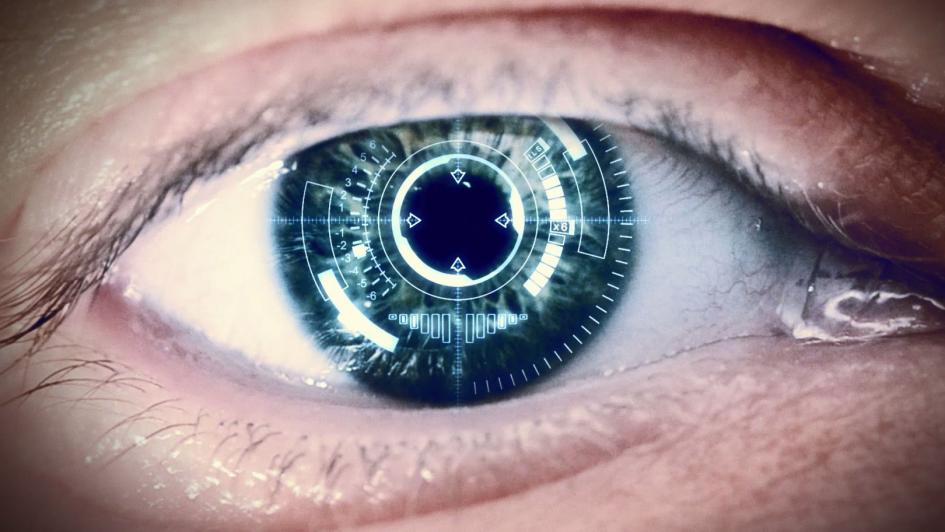
\includegraphics[scale=0.25]{images/contact_lense}
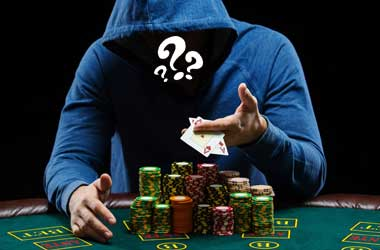
\includegraphics[scale=0.532]{images/poker_player}
\caption{Stock photos of an envisioned camera-equipped contact lense (left) and a mysterious black-jack player (right)}
\end{figure}
\section{Introduction [Daniel \& Frank]}
A big topic in computer vision is the search of methods that are, given a query image, capable of answering questions like: What is present in an image? Is there a particular object in it? Where exactly in the image is this object located? Is it possible to semantically segment objects of interest in the image?
Object detection deals with detecting instances of semantic objects of a certain class (such as humans, buildings, or cars) in digital images and videos. Typically, object detection deals with two sub-taks: \textbf{object localization} using bounding boxes and \textbf{multiclass object classification} within said bounding boxes.
Sometimes, a third sub-task of \textbf{semantic object segmentation} is performed, i.e. the process of labelling objects on pixel level.\\
In this project, we use the YOLOv3 object detection algorithm \cite{DBLP:journals/corr/abs-1804-02767} for object detection (without additional segmentation) in order to tell apart playing cards of a standard 52-part deck.
\newpage
\section{Dataset [Daniel]}
Machine learning is based on the idea of learning patterns in a large number exemplary data in order to build a model that can later perform predictions on unseen test data. For our detection model, we needed to have a large dataset of cards, together with the bounding box information for each of the suit/rank combinations of cards (subsequently referred to as \textit{logos}).  Unfortunately, such a dataset is non-existent, therefore, we decided to create it on our own.  We did this in mainly two big steps, ending up with 750 training images for each card, as well as the necessarily bounding box information.   \\
The first important step was destined to data preparation.  We had to create data and rearrange it in a way that could be easily used for data generation.  Beside this, it was also necessary to detect the convex hulls of the card logos, as they were crucial to get bounding boxes information. We will later expand on why we worked with convex hulls from the start.\\
The second big step was focused on data generation. In order to get datasets that reflect realistic scenarios as good as possible, we randomly applied blurring, changed the lighting and sharpened the cards, pasted them on different textures and finally applied linear transformations on them. Obviously, during all of this, we had to keep track of the convex hulls coordinates. 

\subsection*{Data preparation}
We decided to work with a standard deck of 52 cards, where each card contained two logos.  First, we took 2 different photos for each card, manually cropped the cards to a selection and then rescaled the result to a resolution of 600x900 pixels (as our cards' aspect ratio were 2:3).
For this step, we used the selection/rotation/cropping/rescale -tools provided by GIMP\footnote{GIMP 2.8.22 - GNU Image Manipulation Program}. \\
Concluding this, we proceed by detecting the convex hulls of the card logos. We used the python libraries SciPy\footnote{SciPy: Open Source Scientific Tools for Python} and OpenCV\footnote{OpenCV: Open Source Computer Vision Library} to obtain the desired detections in a semi-automatic way (Figure \ref{fig-data-prep} illustrates this process). After verifying each manually selection, we saved the two convex hulls of each card as an NumPy array. The above procedure is outlined in Figure 2.\\
\\ \\
\begin{minipage}{\columnwidth}
\makeatletter
\newcommand{\@captype}{figure}
\makeatother
\centering
\captionsetup[subfigure]{labelformat=empty}
\subfloat[\scriptsize Queen of spades with a resolution of 600x900 pixels.]{%
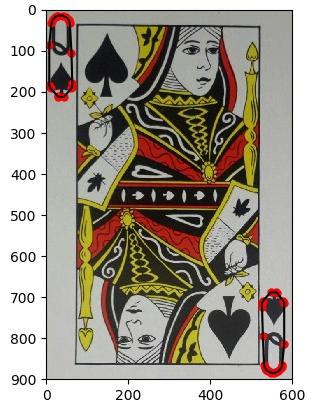
\includegraphics[scale=0.587]{images/qs_2}%
} \qquad \qquad%
\subfloat[\scriptsize Detected convex hulls.  The red points were saved as a NumPy array.]{%
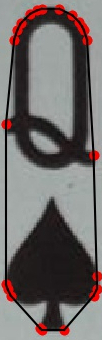
\includegraphics[scale=0.68]{images/qs_2_1} \quad
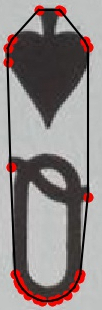
\includegraphics[scale=0.74]{images/qs_2_2}  }
\caption{Semi automatic detection of the convex hulls.}
\label{fig-data-prep}
\end{minipage}
\newpage
\subsection*{Synthesize a general dataset}
With all the images in the same resolution and having detected the bounding boxes for each card, the next goal was to generate a big amount of new data destined to train our model. \\
First, we randomly blurred the cards using Gaussian, average and median filters.  We also randomly performed sharpening and lighting operations on the image.  After this, we pasted the cards in the middle of large textures using the describable textures dataset \cite{cimpoi14describing}.
In total, we pasted each card onto 75 different textures destined for the training and in 15 different textures for testing (the textures used for train/test were not mutually exclusive).  Figure \ref{fig-canvas} illustrate some examples and textures. \\ \\

\begin{minipage}{\columnwidth}
\makeatletter
\newcommand{\@captype}{figure}
\makeatother
\centering
\captionsetup[subfigure]{labelformat=empty}
\subfloat[ ]{%
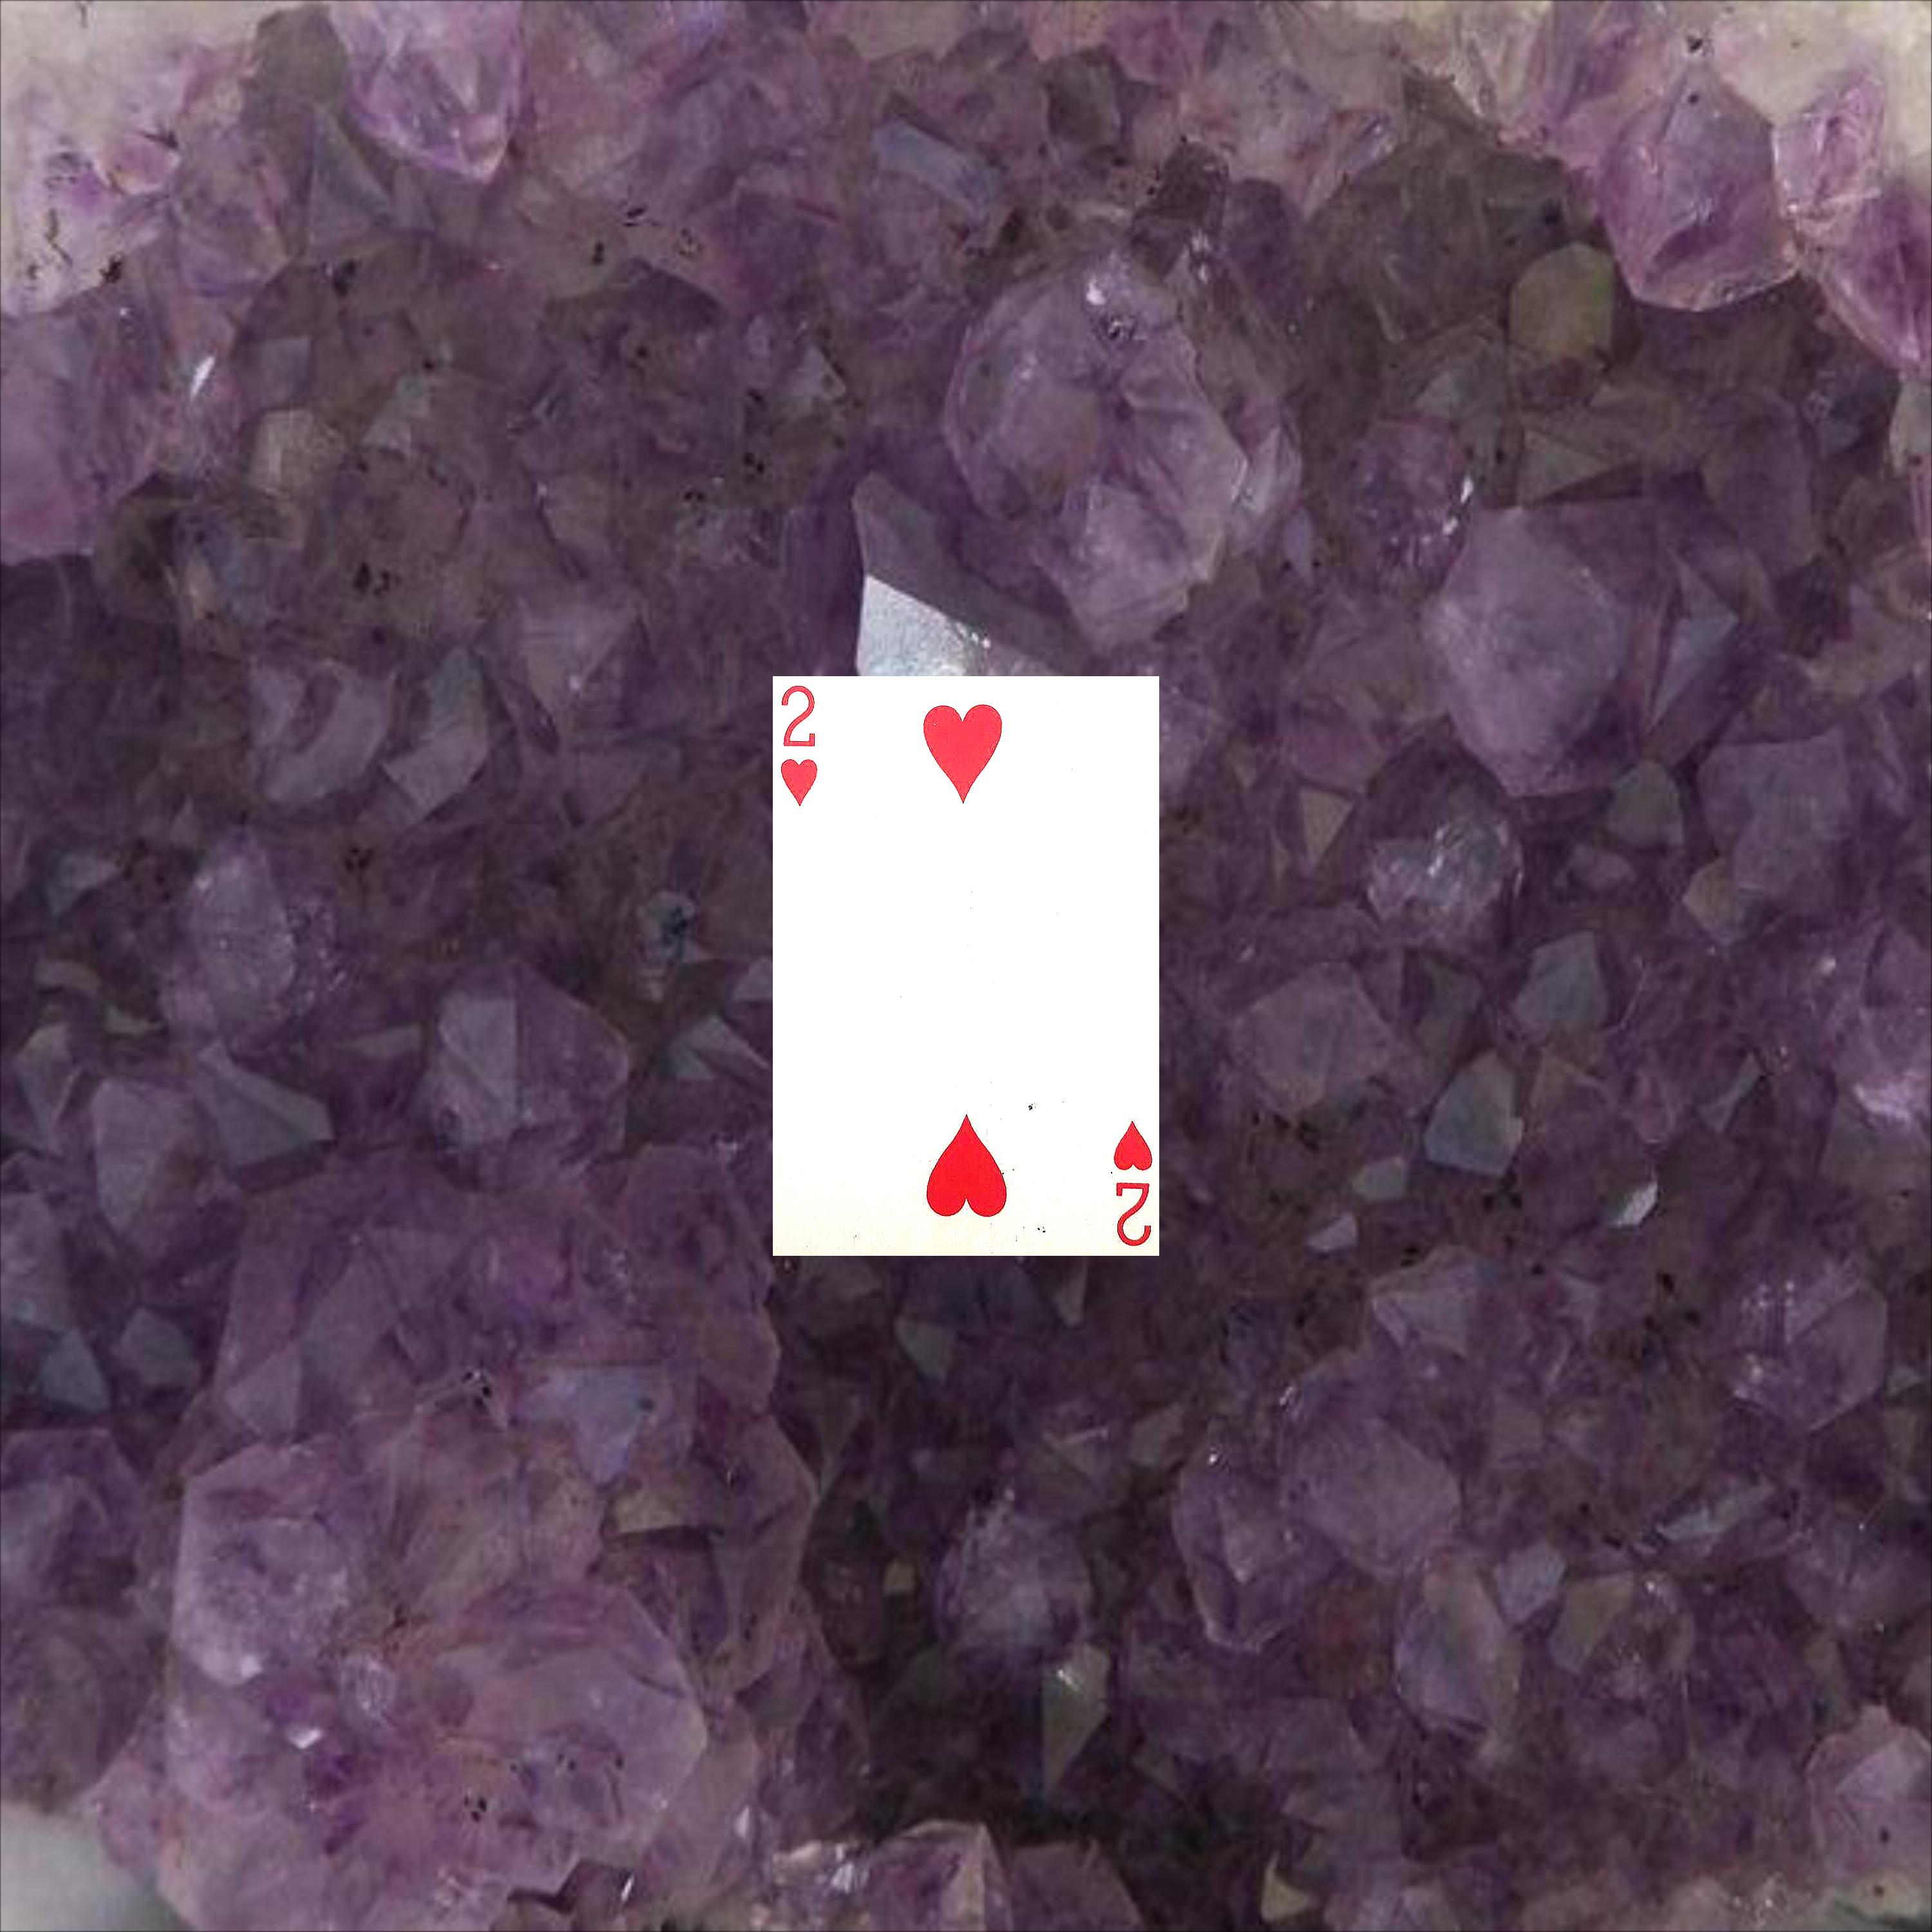
\includegraphics[scale=0.04]{images/2h_1}  \quad%  
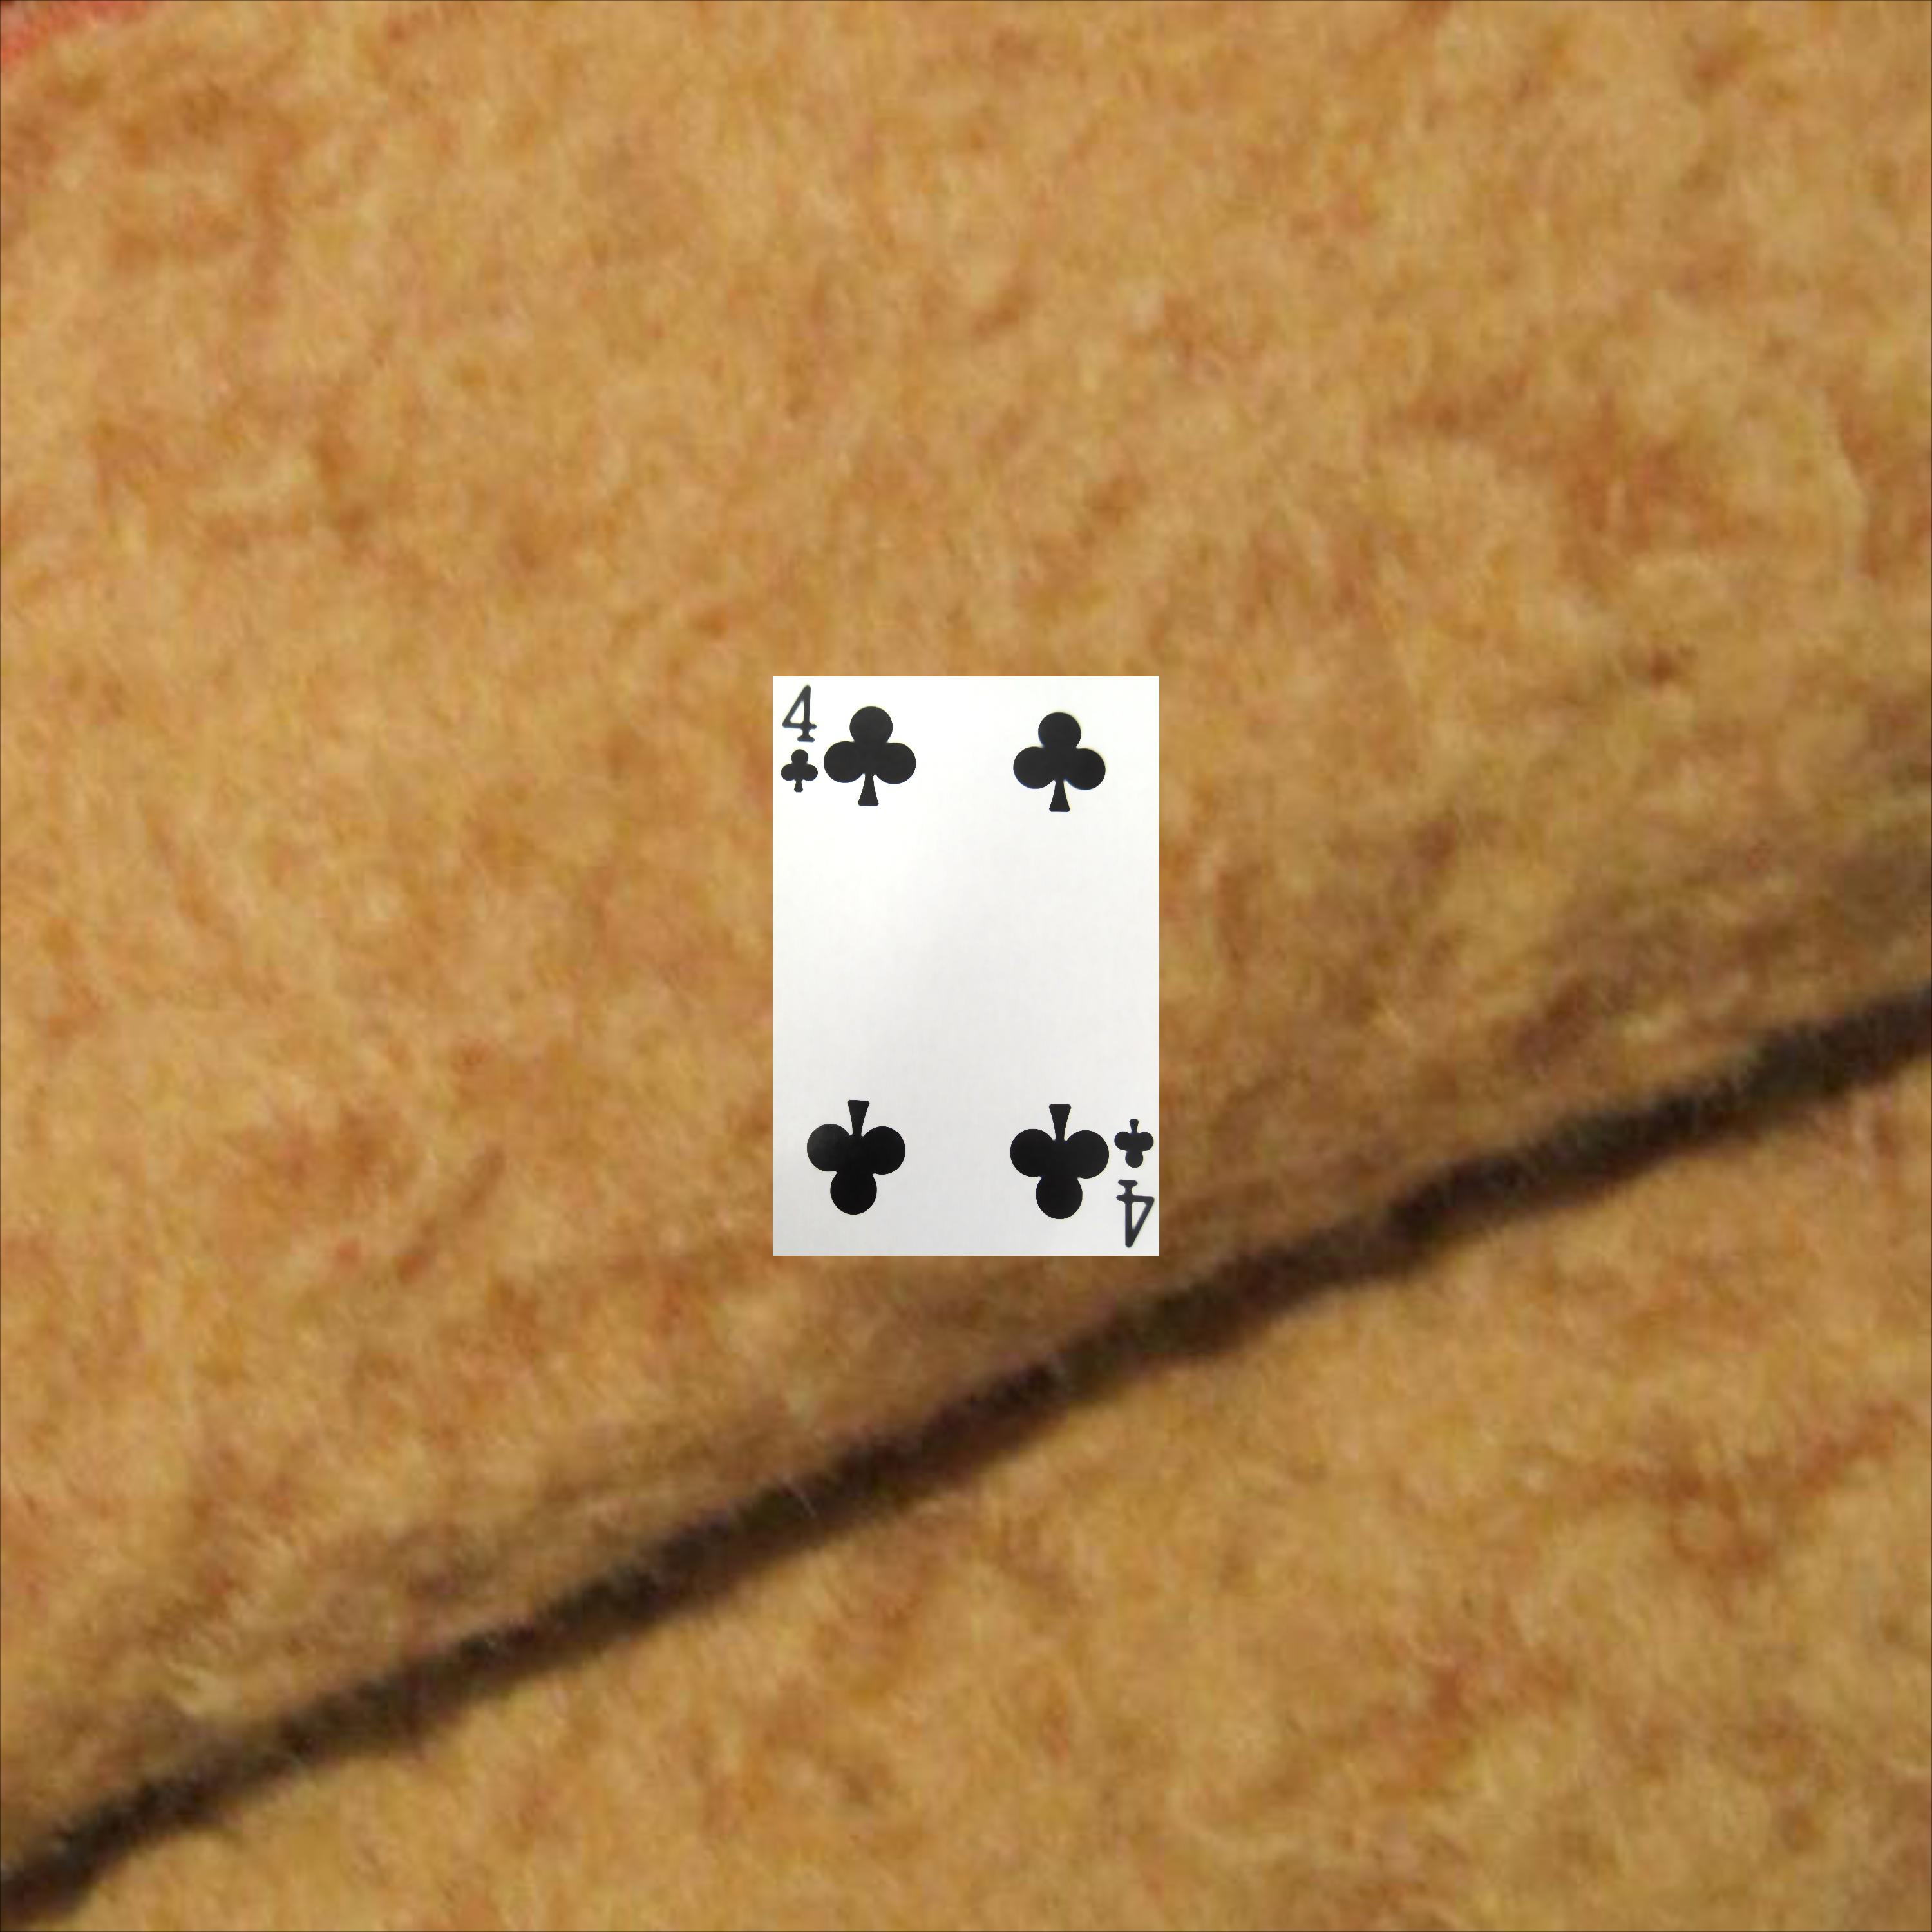
\includegraphics[scale=0.04]{images/4c_1}  \quad%  
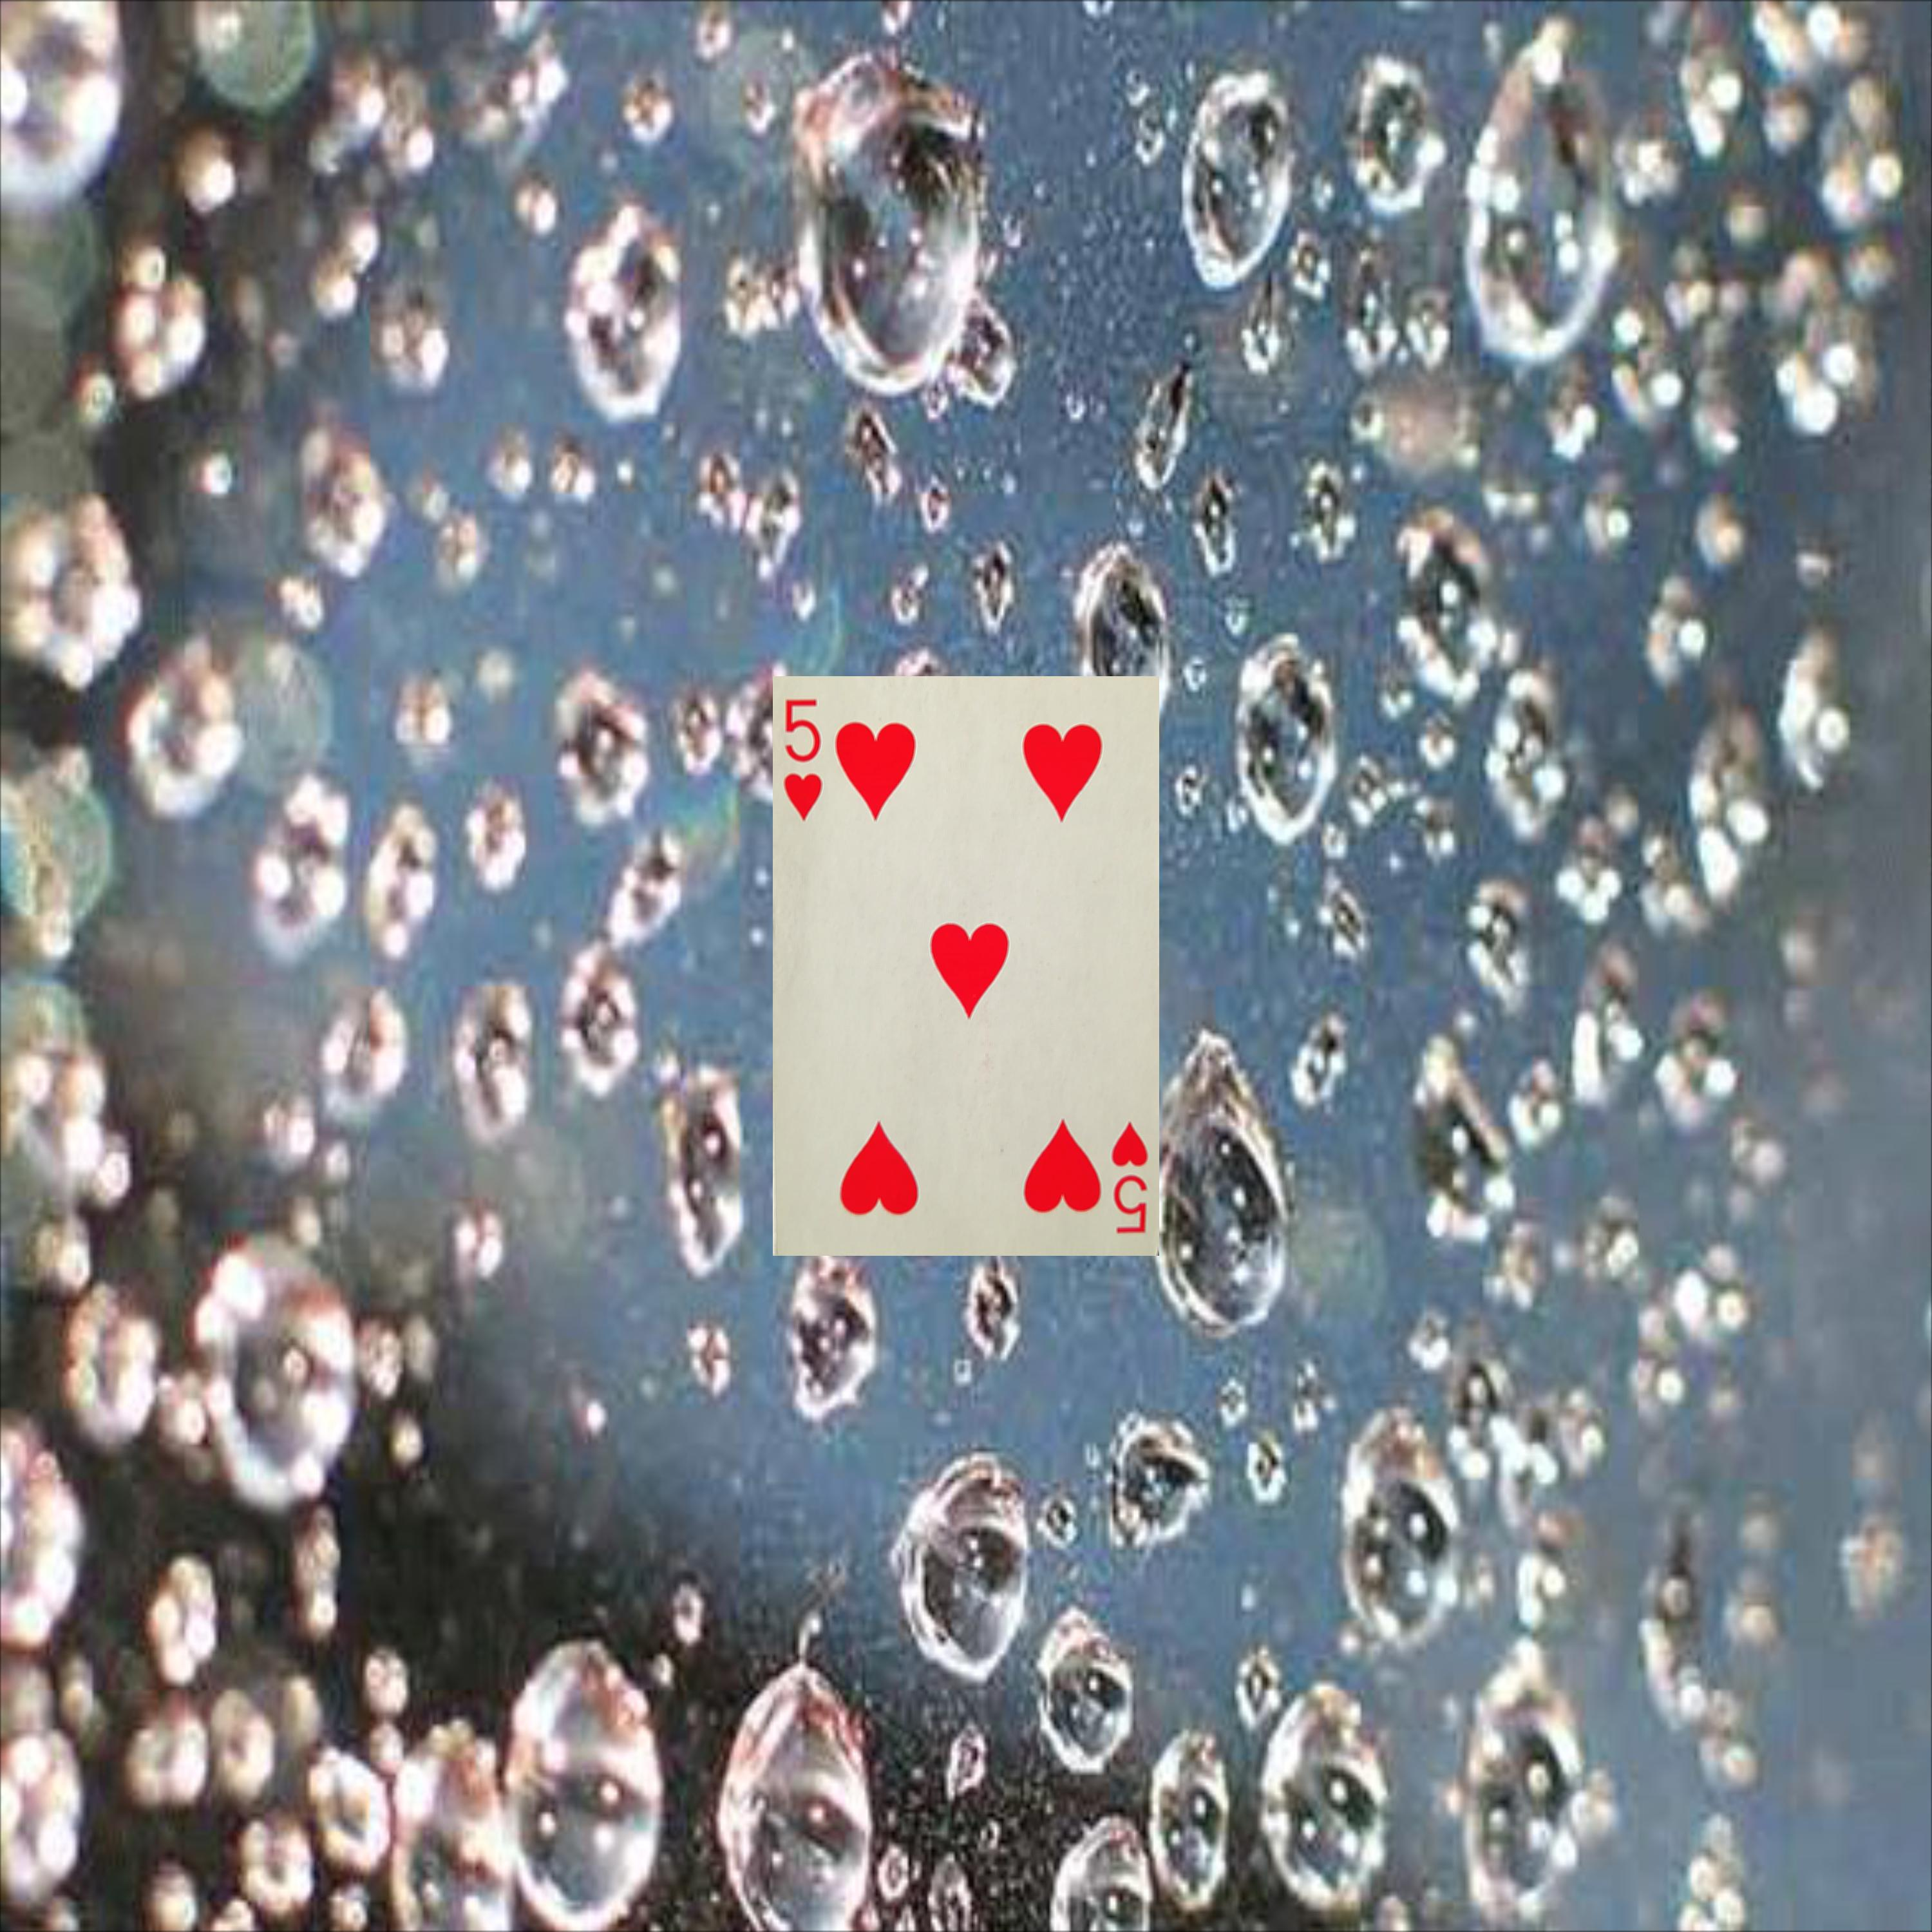
\includegraphics[scale=0.04]{images/5h_1}}  \qquad 
\subfloat{%
\vspace{1cm}
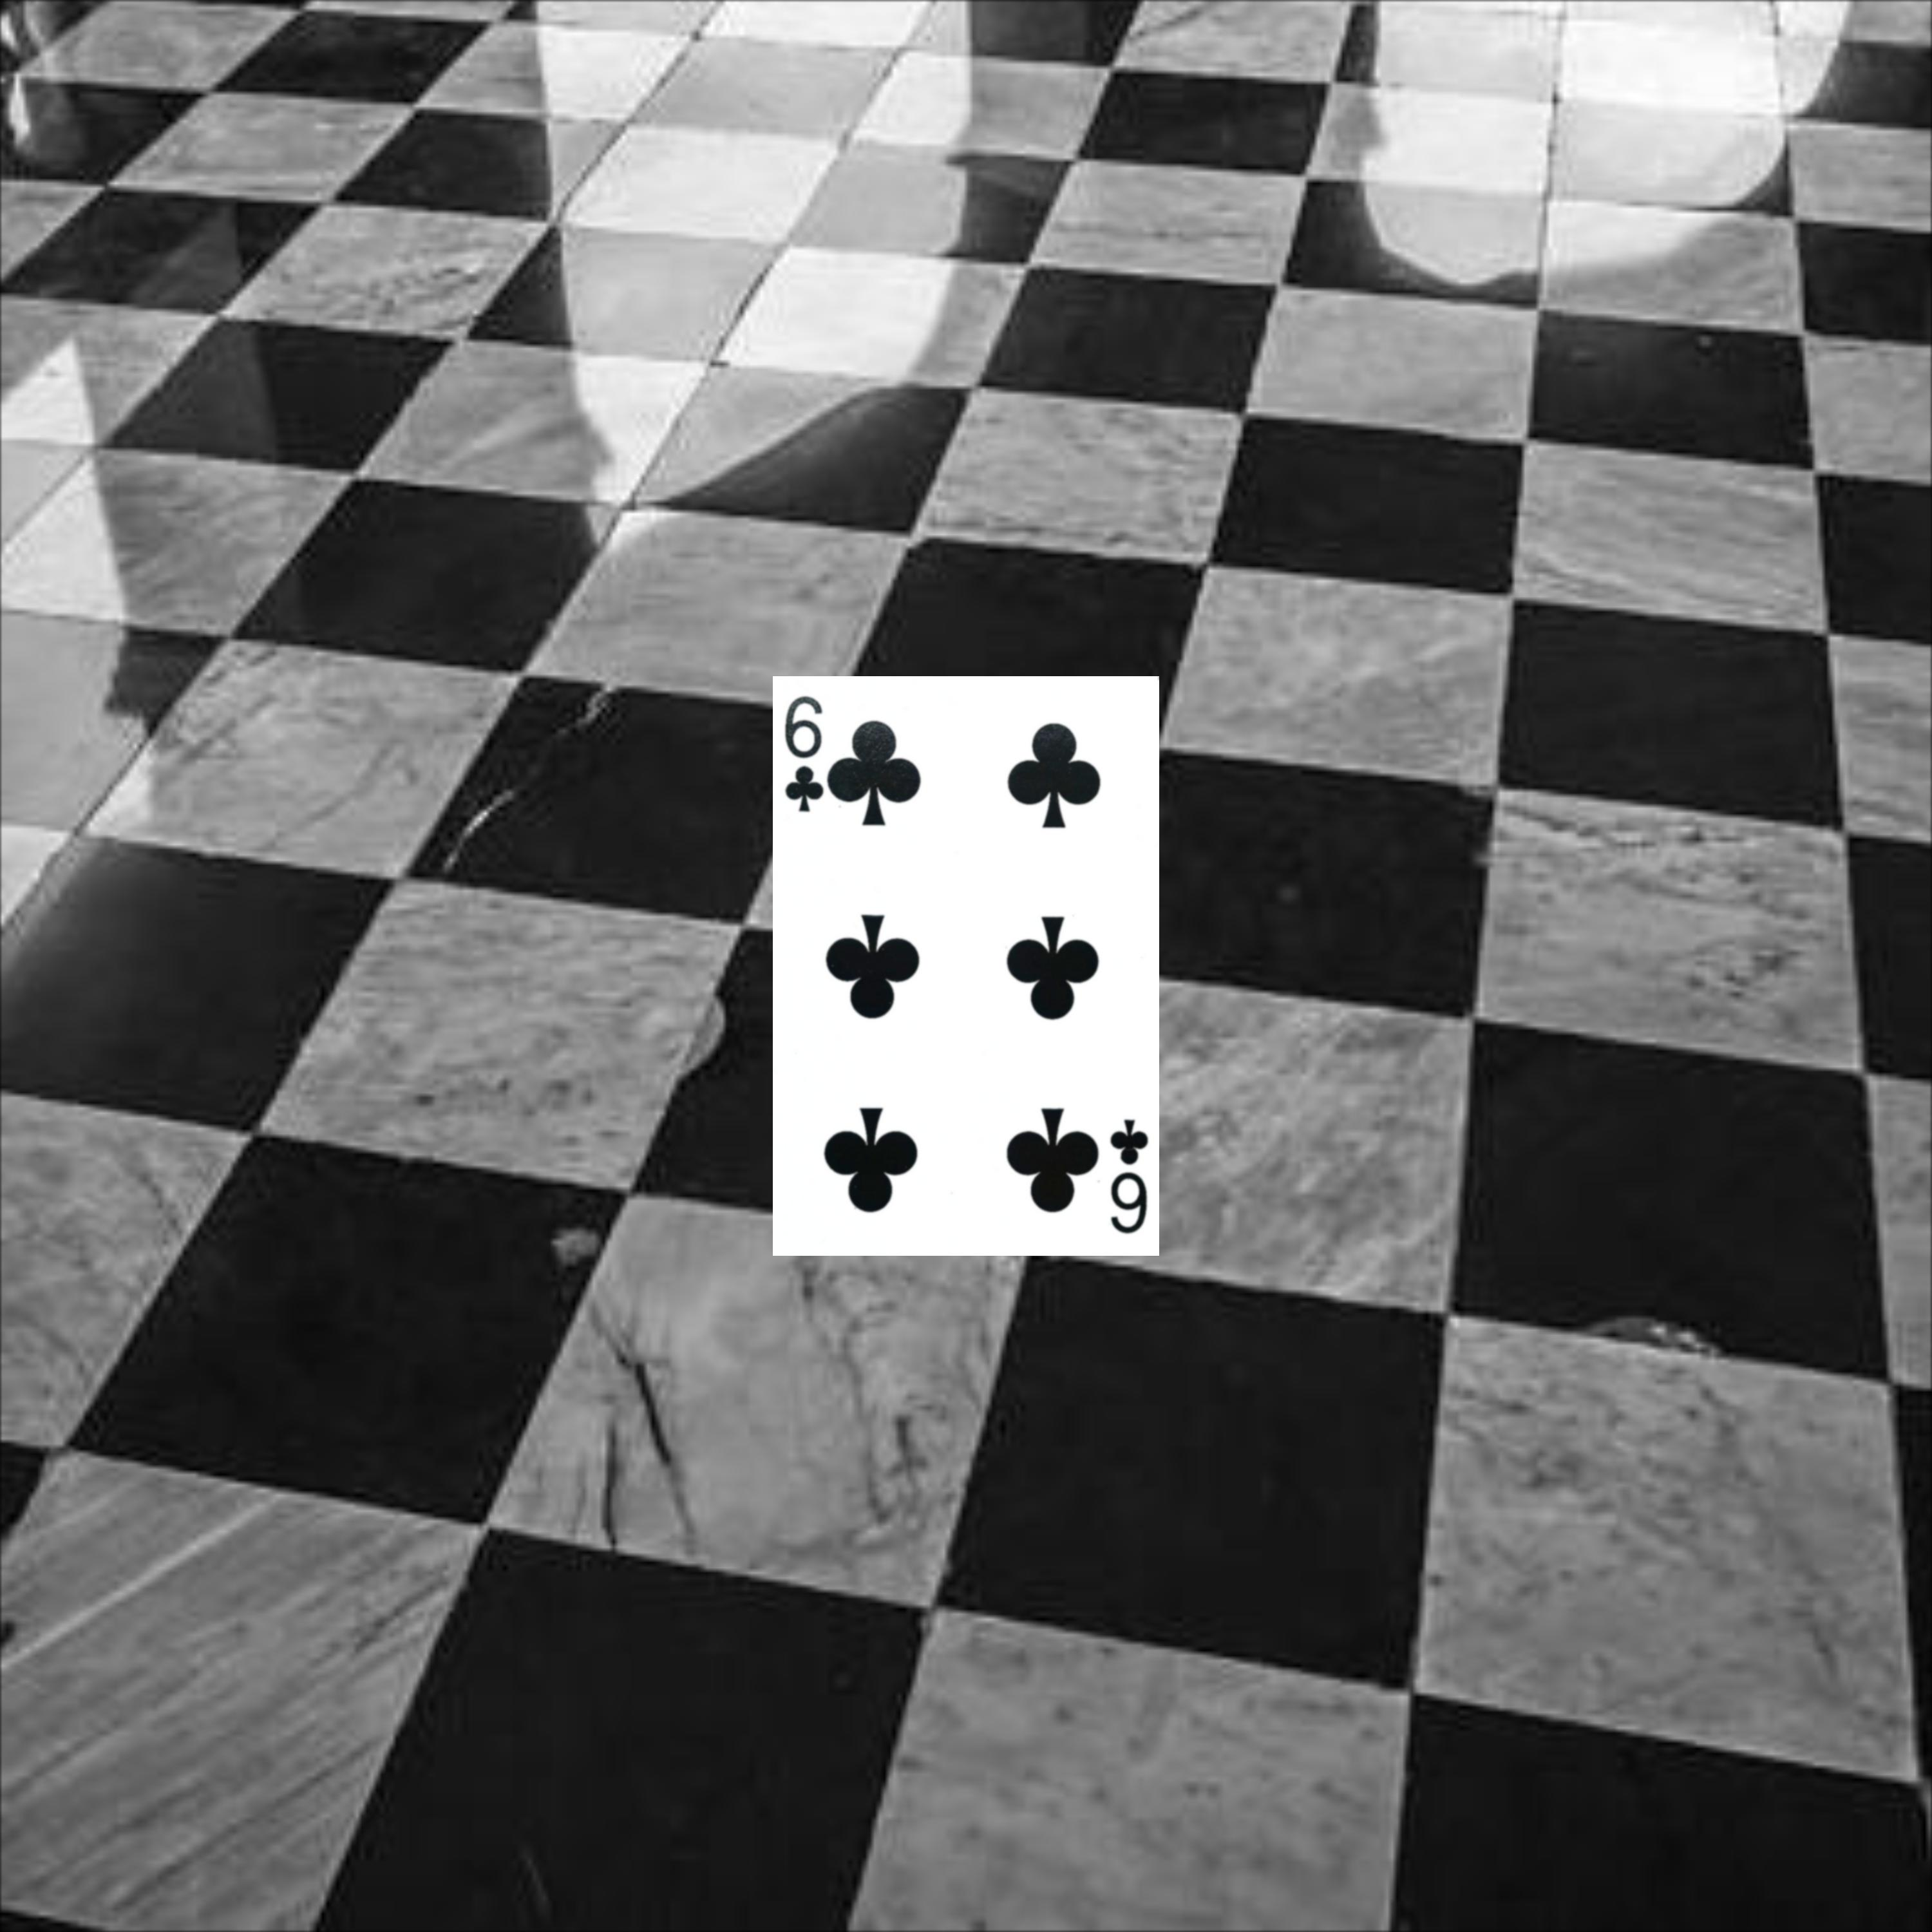
\includegraphics[scale=0.04]{images/6c_1}  \quad%  
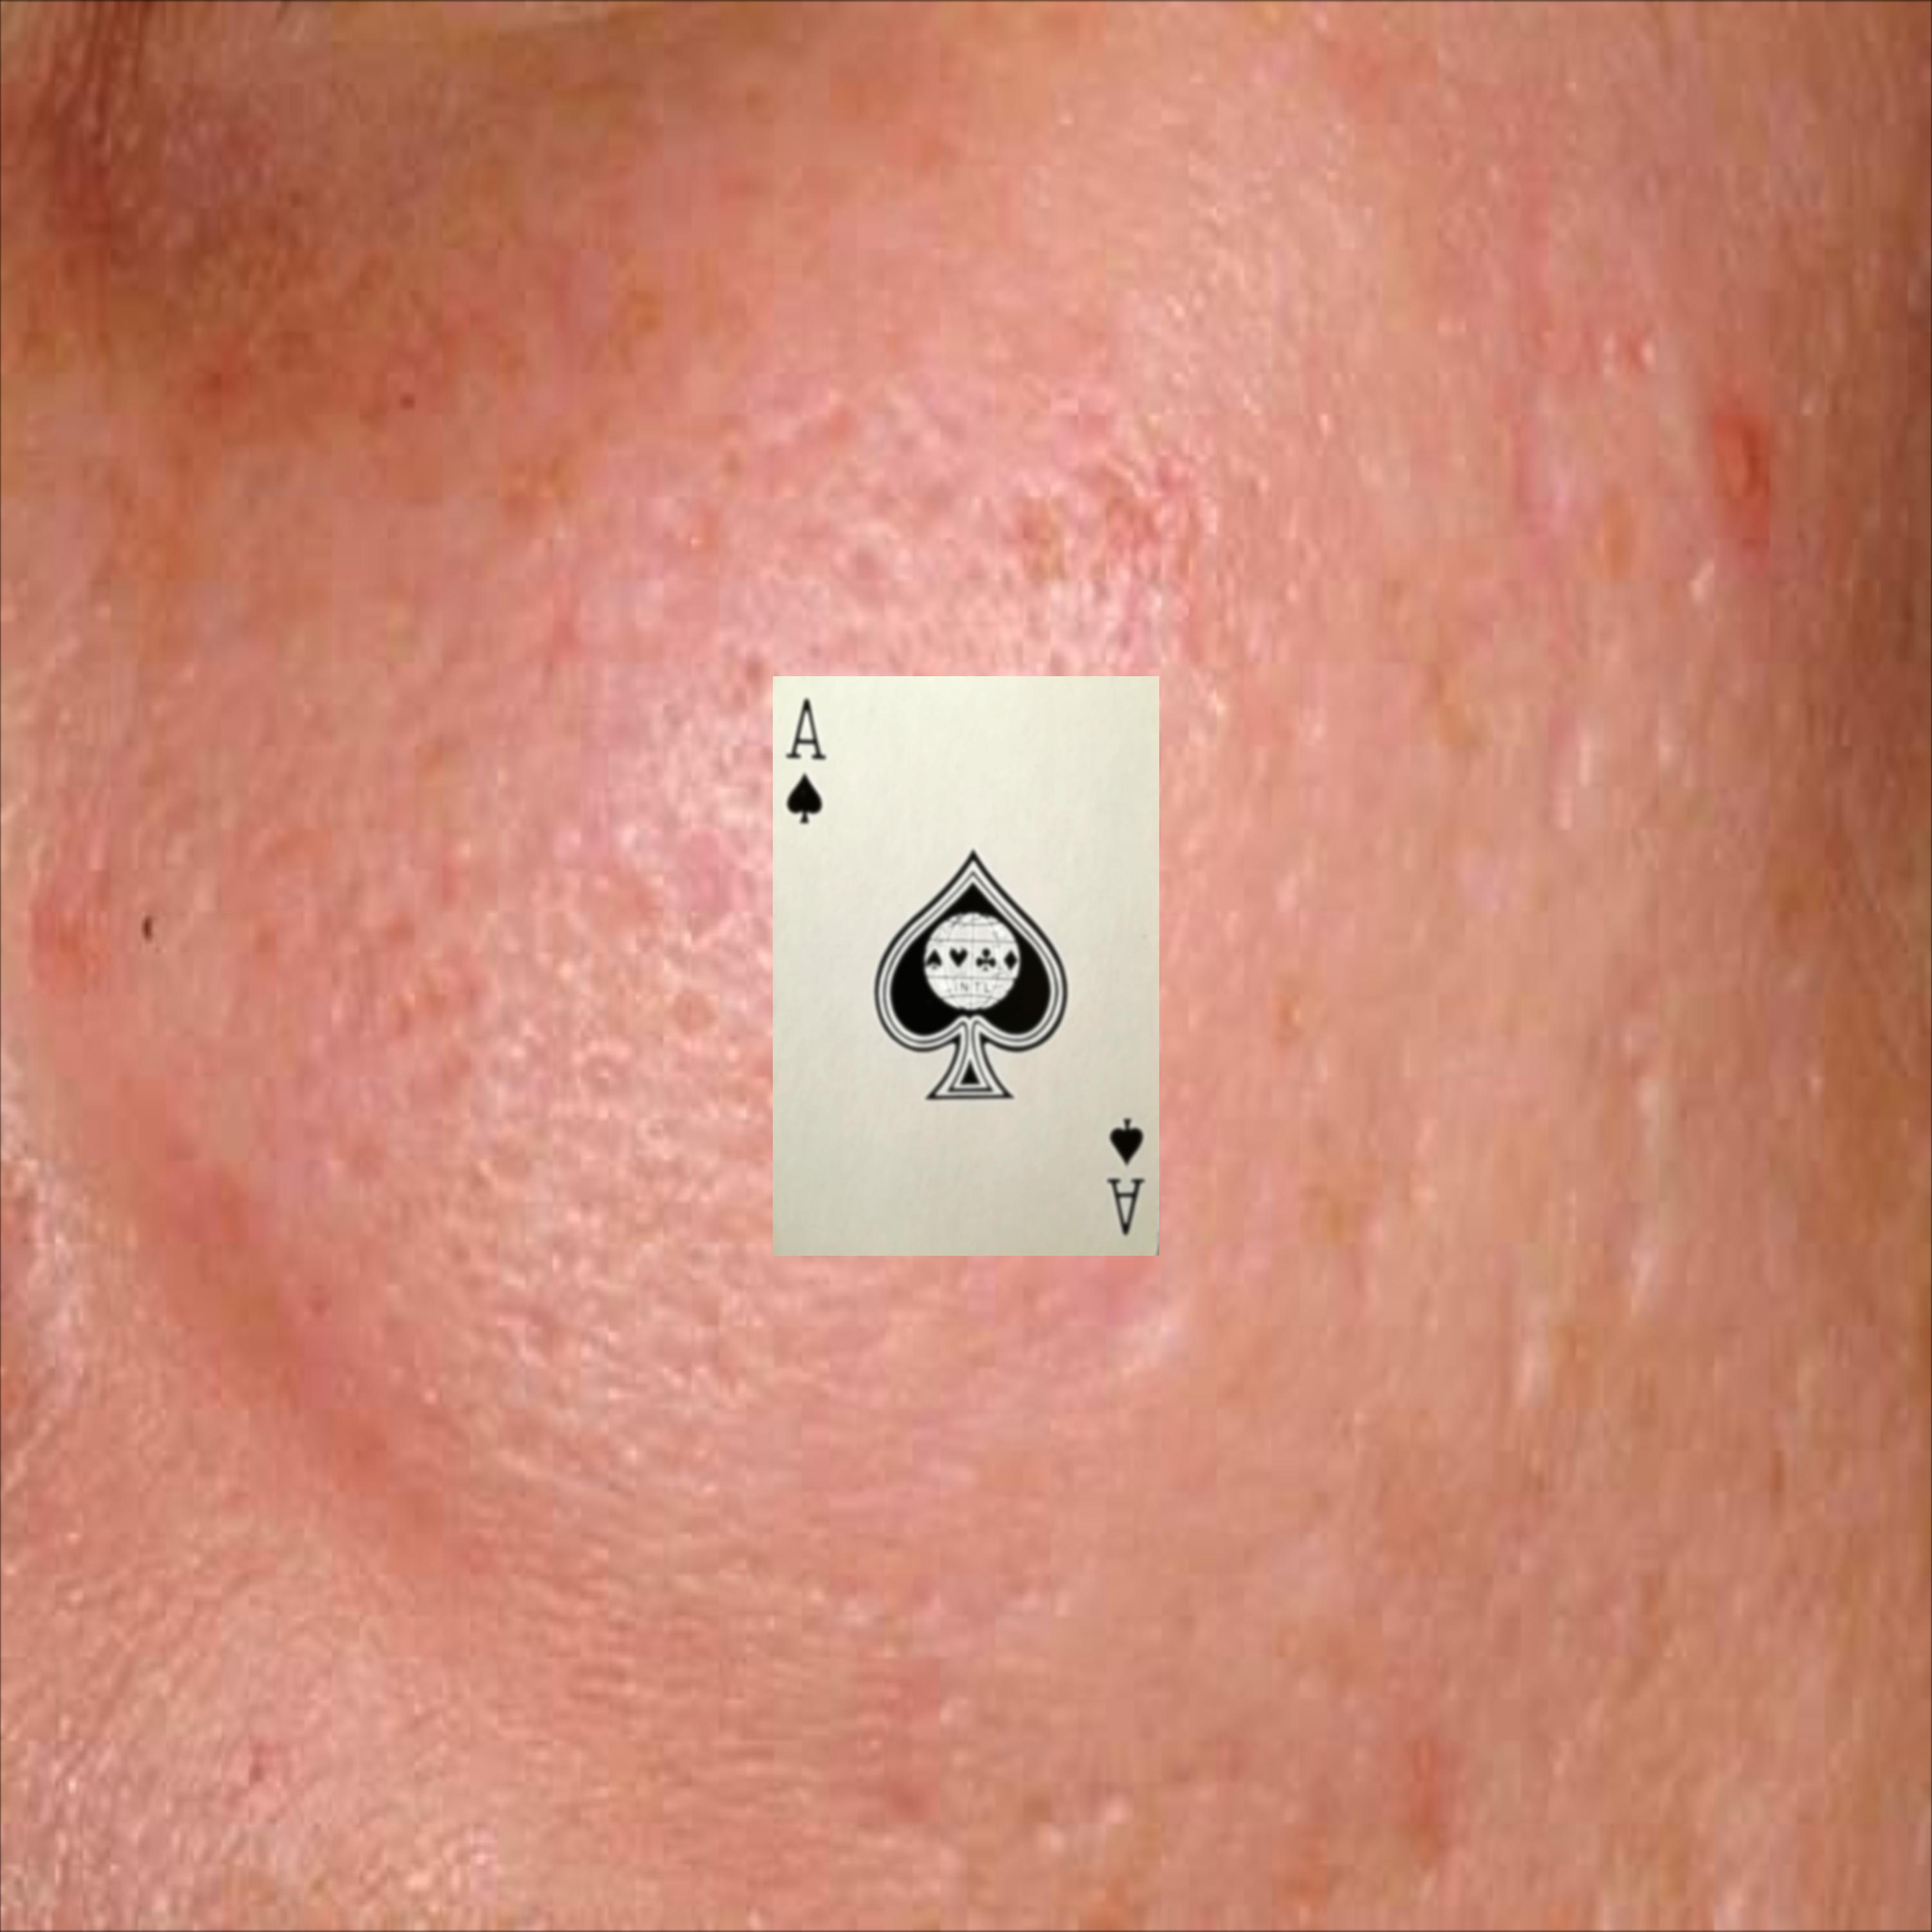
\includegraphics[scale=0.04]{images/as_1}  \quad
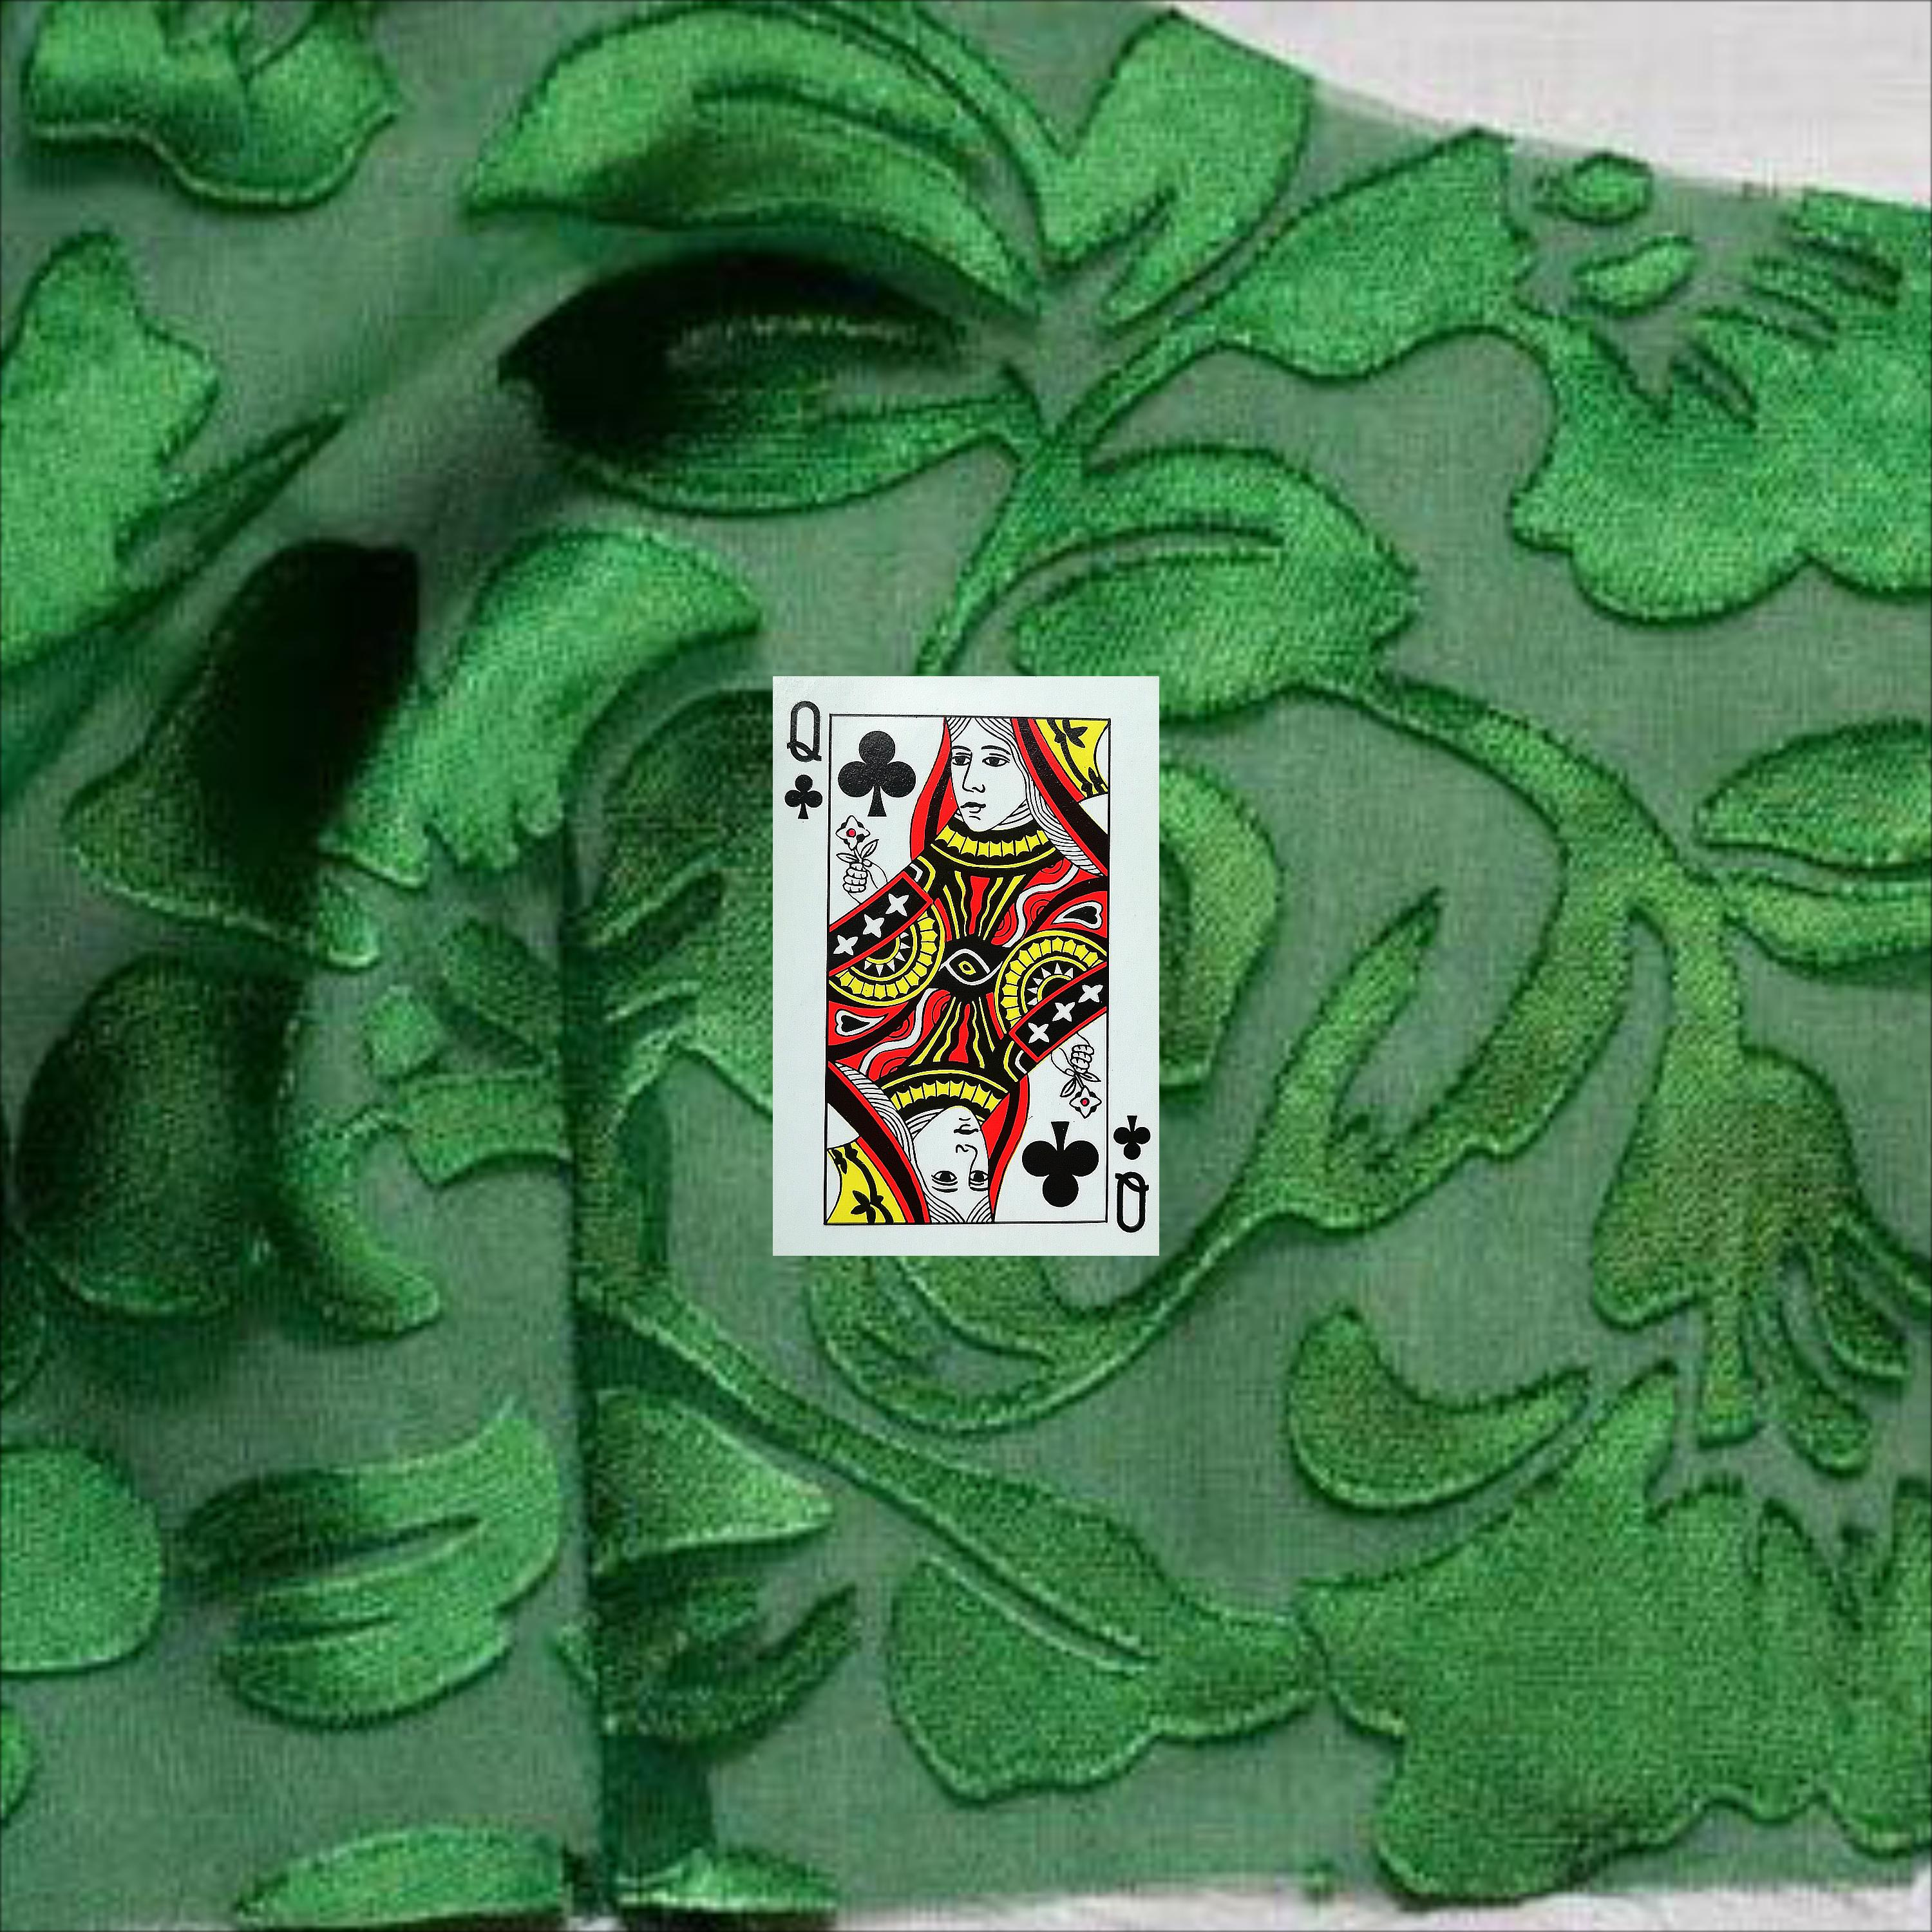
\includegraphics[scale=0.04]{images/qc_1} }
\caption{Some cards pasted into canvases of 3000x3000 pixels.}
\label{fig-canvas}
\end{minipage}
\newline \newline\newline 
\noindent As a next step in data synthesis, we performed transformations with images such as the above. We performed scaling, translation and rotation using randomized parameters using the imgaug\footnote{http://imgaug.readthedocs.io/en/latest/} python library.  Concluding this, we crop the images to the middle, reducing their pixel resolution to 800 $\times$ 800 pixels. This operation allowed us to easily obtain the realistic scenario of partially occluded cards. However, cropping also led the partially/complete lost of some convex hulls Therefore, we only kept  convex hulls that had enough points left in the image using thresholding rules.  
Figure \ref{img-cards examples} displays a number of situations that might occur. \\
The \textbf{imgaug} python library turned out to be a very useful tool for our dataset creation pipeline because it allowed us to keep track of the convex hulls easily.

\begin{minipage}{\columnwidth}
\makeatletter
\newcommand{\@captype}{figure}
\makeatother
\centering
\captionsetup[subfigure]{labelformat=empty}

\subfloat[]{%
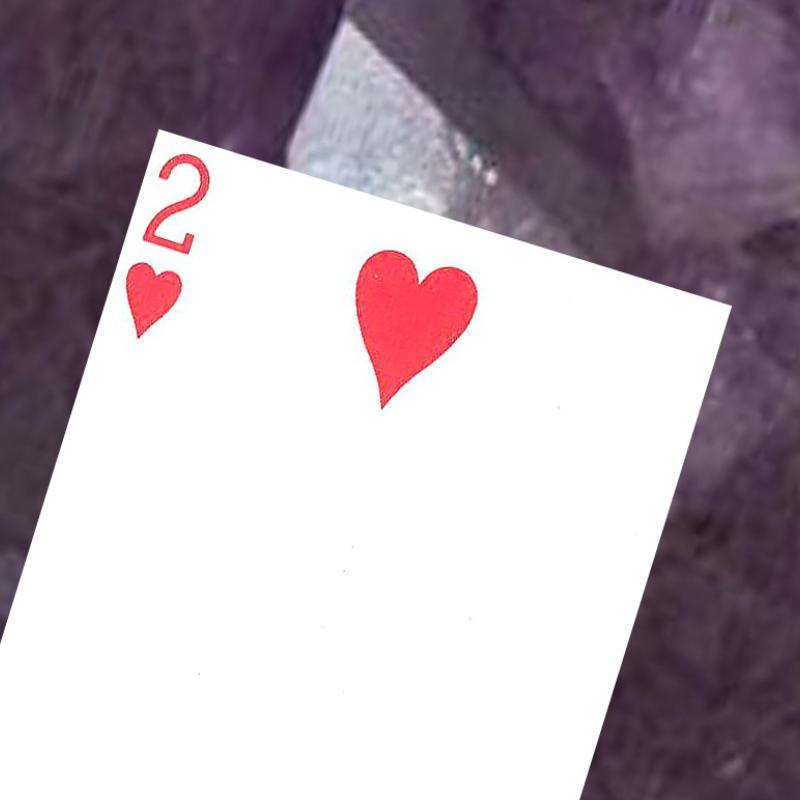
\includegraphics[scale=0.1]{images/2h_2}  \ 
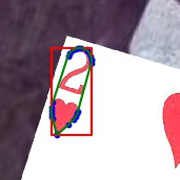
\includegraphics[scale=0.615]{images/2h_4}}  
\qquad
\subfloat{%
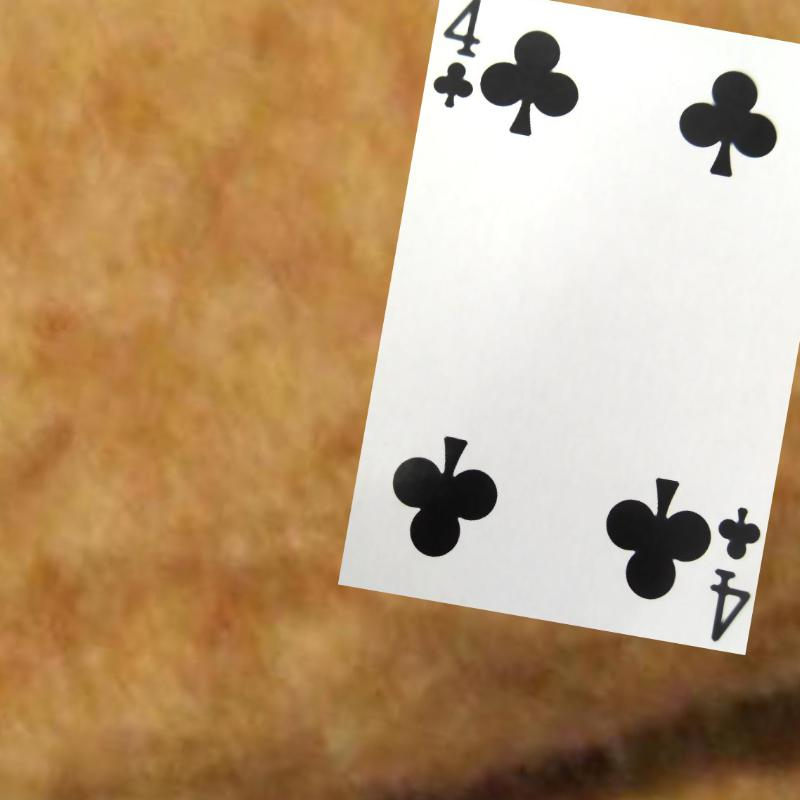
\includegraphics[scale=0.1]{images/4c_2}  \  
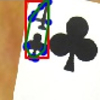
\includegraphics[scale=1.12]{images/4c_4}}  
\qquad
\subfloat{%
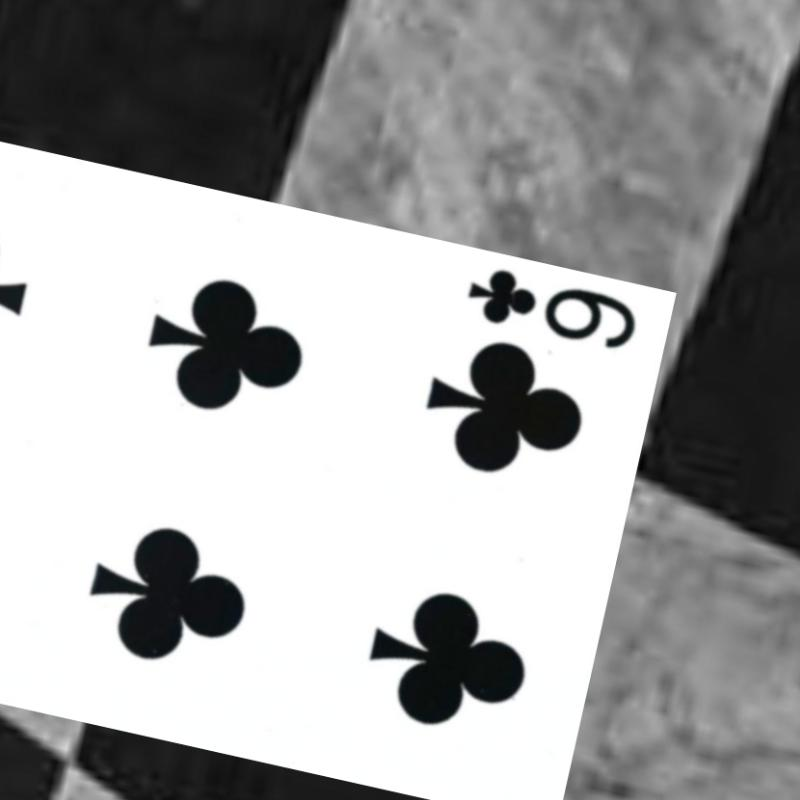
\includegraphics[scale=0.1]{images/6c_2}  \
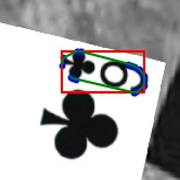
\includegraphics[scale=0.615]{images/6c_4}}  
\qquad
\subfloat[]{%
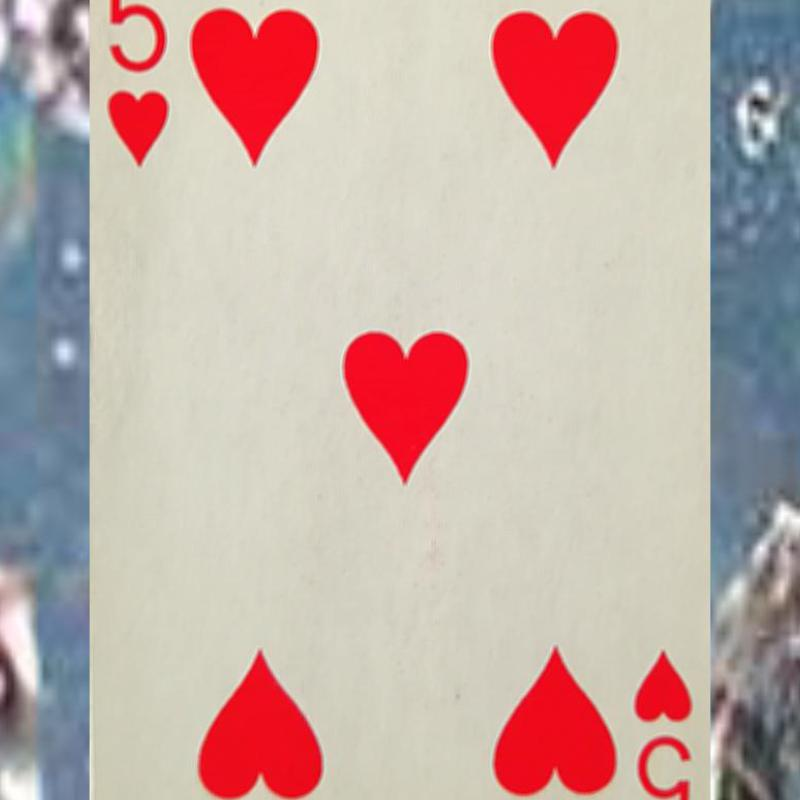
\includegraphics[scale=0.1]{images/5h_2}  \
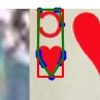
\includegraphics[scale=1.12]{images/5h_4}}  
\qquad
\subfloat{%
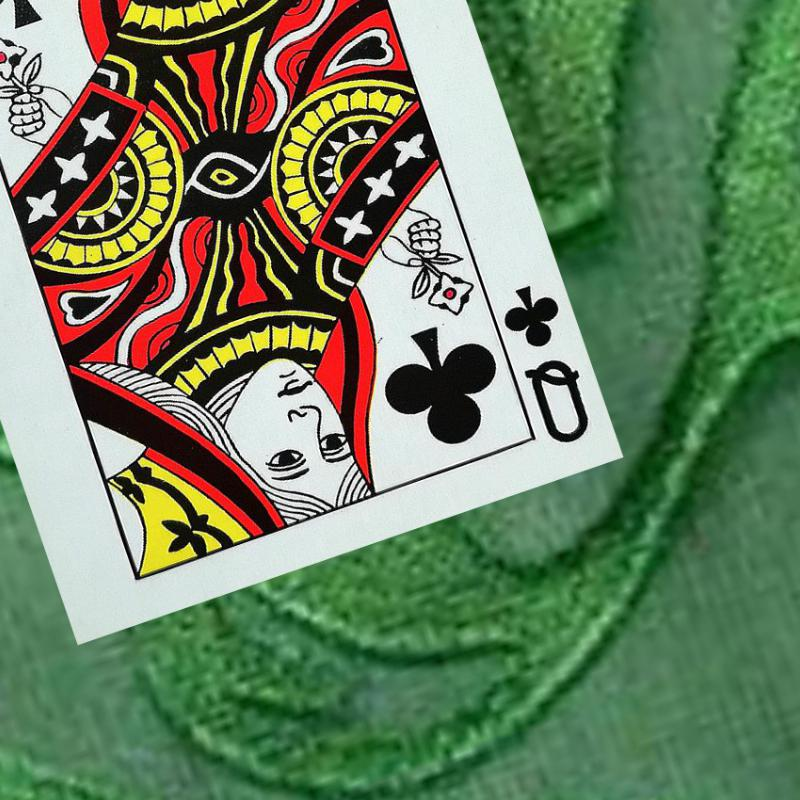
\includegraphics[scale=0.1]{images/qc_2}  \
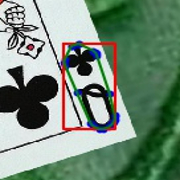
\includegraphics[scale=0.615]{images/qc_4}}  
\qquad
\subfloat{%
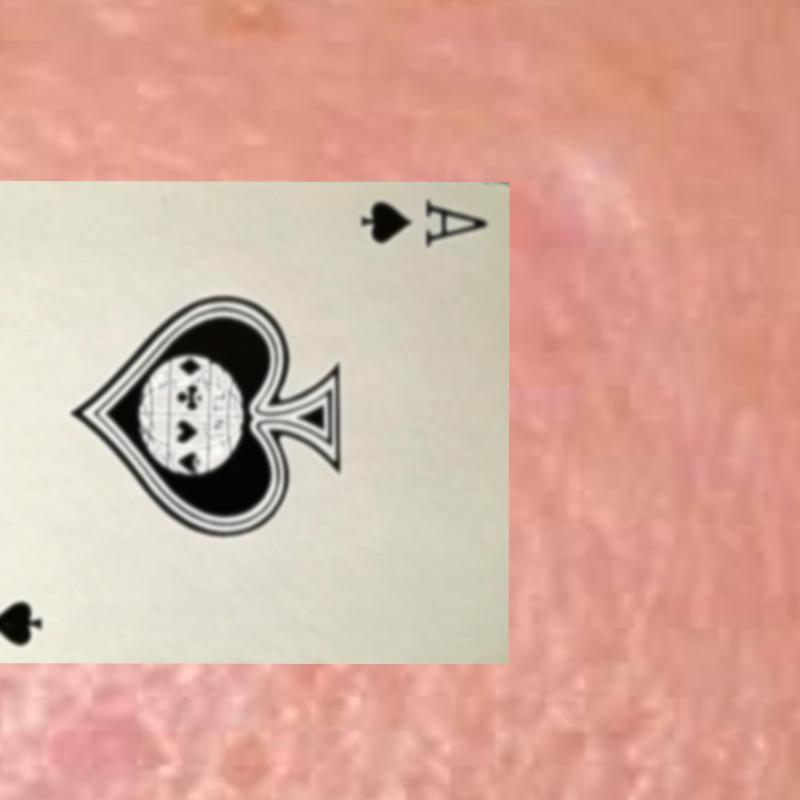
\includegraphics[scale=0.1]{images/as_2}  \
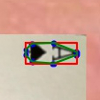
\includegraphics[scale=1.12]{images/as_4}}  
\qquad
\caption{Images of the previous paragraph after randomly performed transformations.}
\label{img-cards examples}
\end{minipage}

\subsection*{The convex hull approach}
YOLOv3 expects a \textit{.txt}-file for each image, with a line for each ground truth object in the image that looks like:
<object-class><x><y><width><height>, where x, y are the center positions of the bounding boxes (BBs) and the width and height, also of the BBs, are relative to the images' width and height.  
As is always the case, bounding boxes are perpendicular/aligned with image borders and can't be rotated. Nevertheless, we can rotate the edge coordinates of bounding boxes around. This would, however, lead to bounding boxes that are ` ``larger than necessary'' (Figure \ref{bb-ch} illustrates this problem).\\
Using convex hulls to keep track of logos, we always obtain minimal bounding boxes. 

%\begin{minipage}{\columnwidth}
%\makeatletter
%\newcommand{\@captype}{figure}
%\makeatother
%\centering
%\captionsetup[subfigure]{labelformat=empty}
%\subfloat[0]{%
%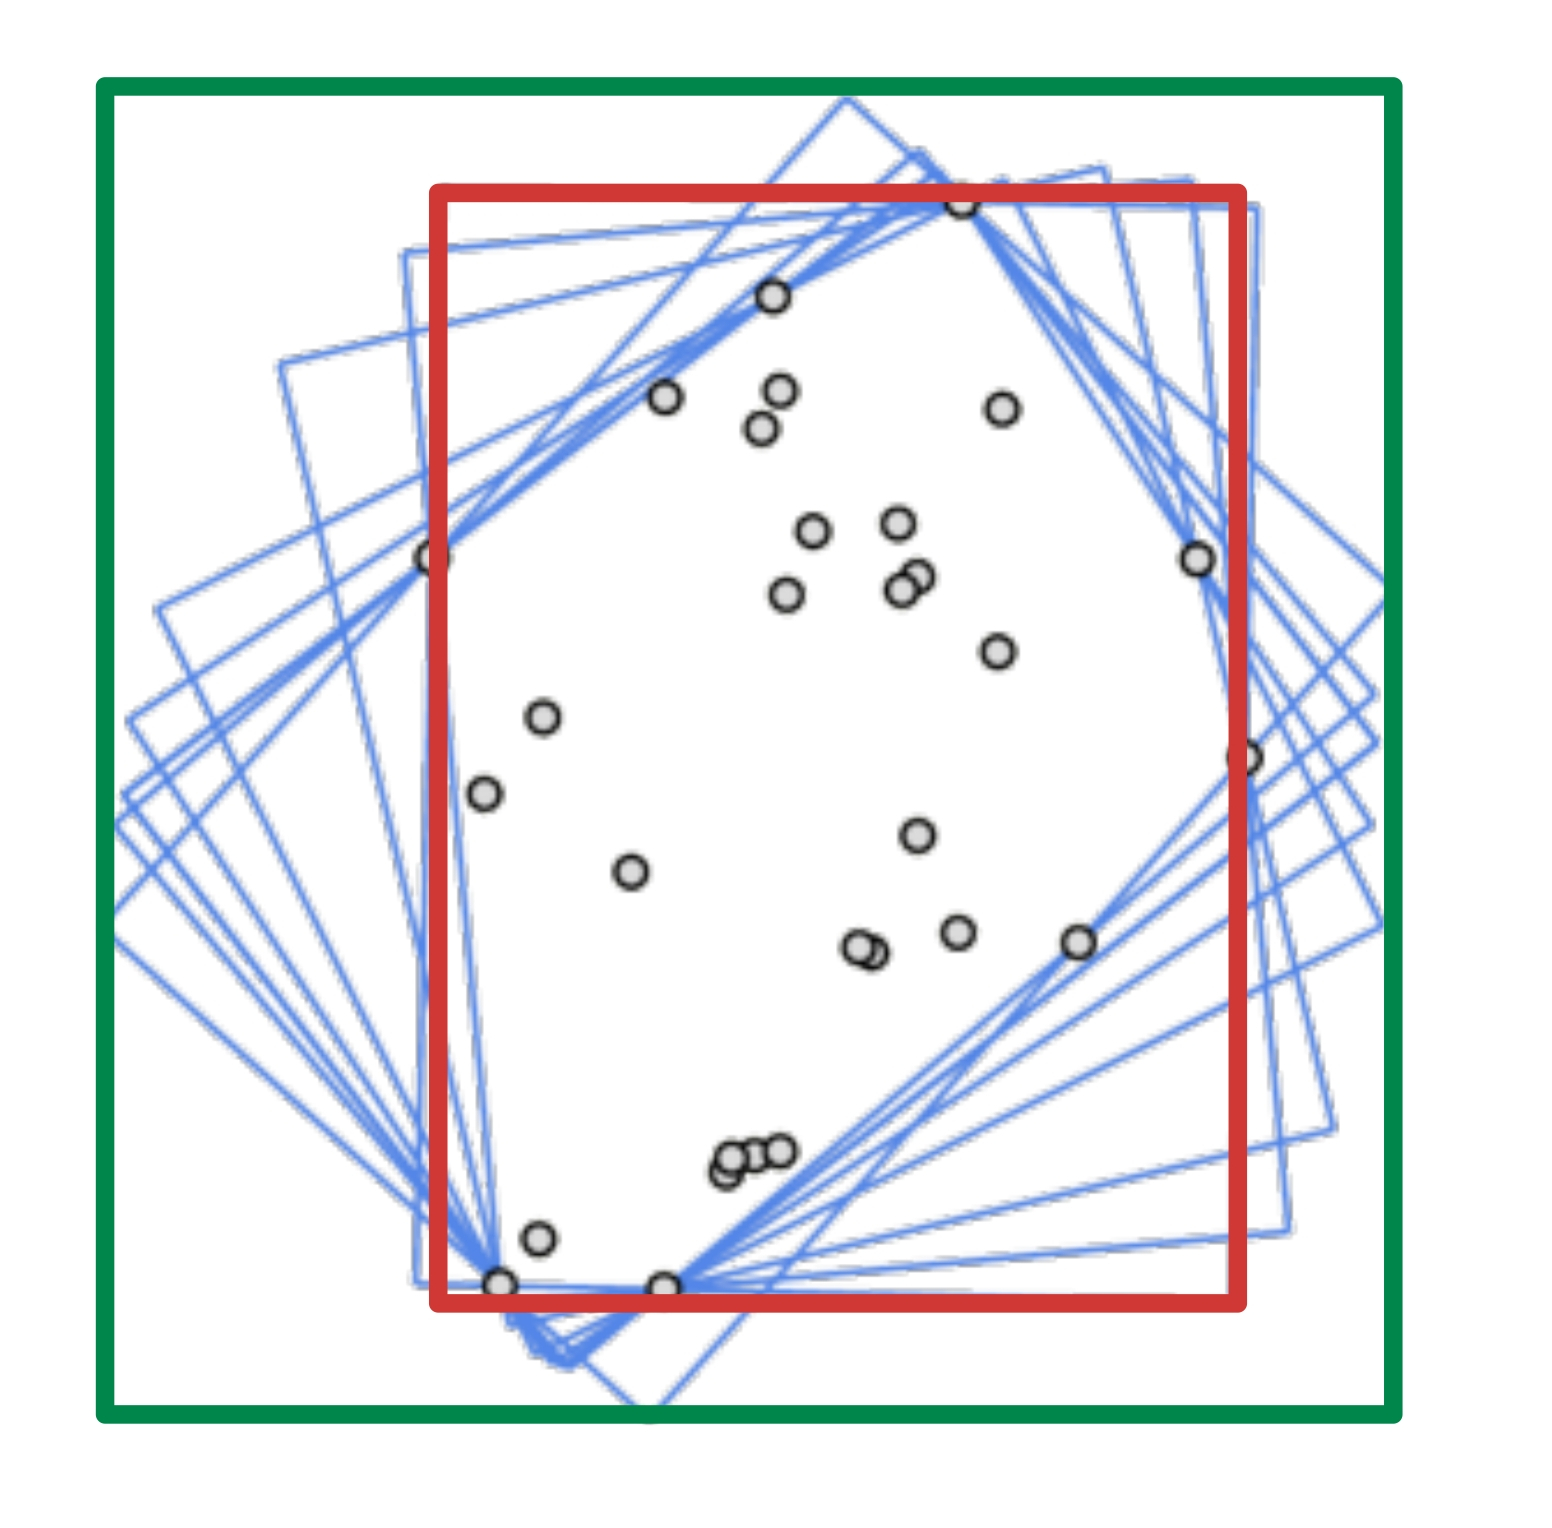
\includegraphics[scale=0.19]{images/ch_vs_bb}  }
%\caption{Green box represents the BB when applying some rotations, while the red box represents the BB of the convex hull.}
%\label{bb-ch}
%\end{minipage}

\begin{figure}[h]
\centering
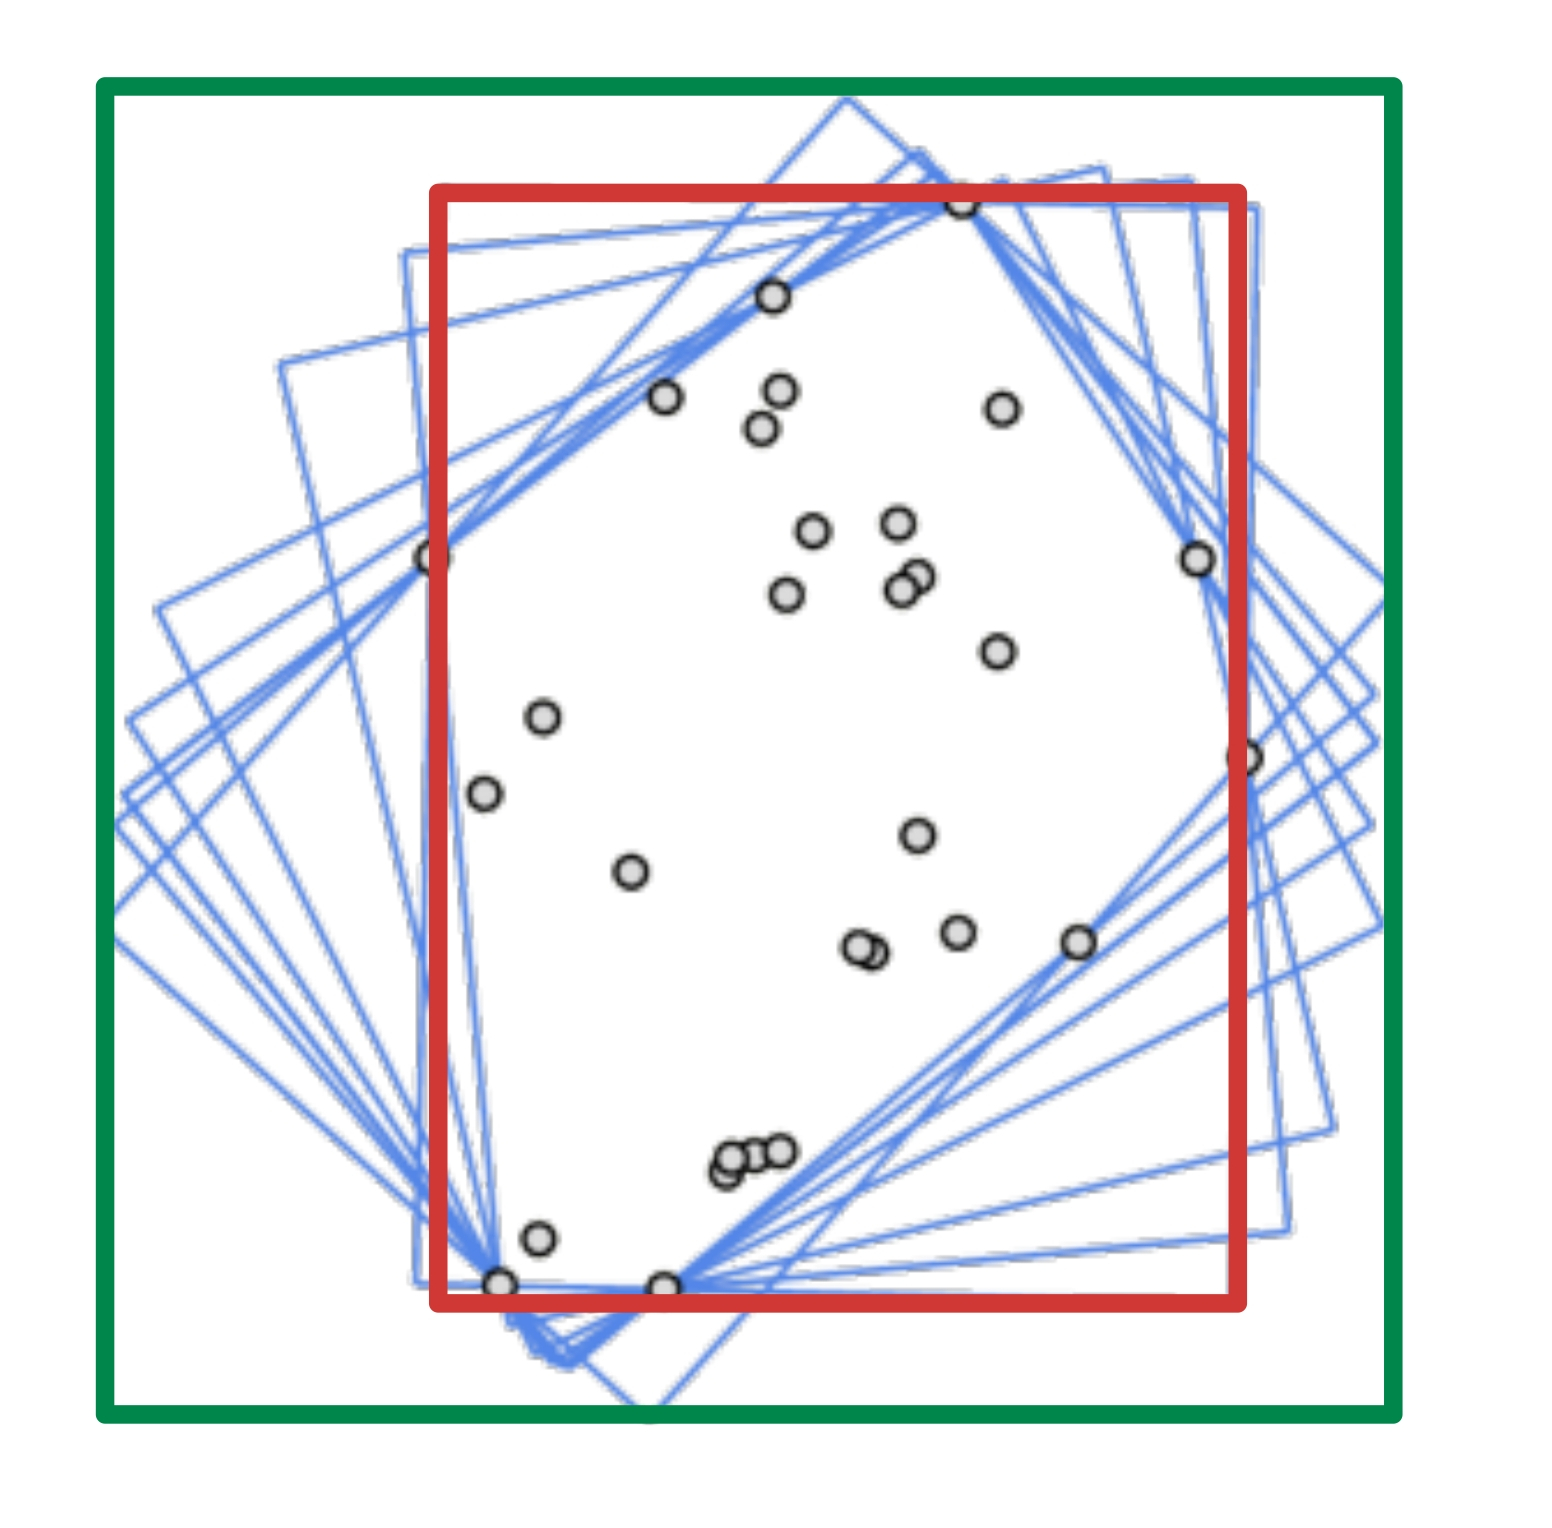
\includegraphics[scale=0.15]{images/ch_vs_bb} 
\caption{The green box represents the ``worst case'' BB after applying some rotations, while the red box represents the BB of the convex hull.}
\label{bb-ch}
\end{figure}

\section{Related work - The object detection landscape [Frank]}
The task of object detection in images encompasses both localizing objects using bounding boxes and subsequently classifying objects within these bounding boxes.

For these tasks, different deep learning architectures have emerged, of which 

\begin{wrapfigure}{l}{0.48\textwidth}
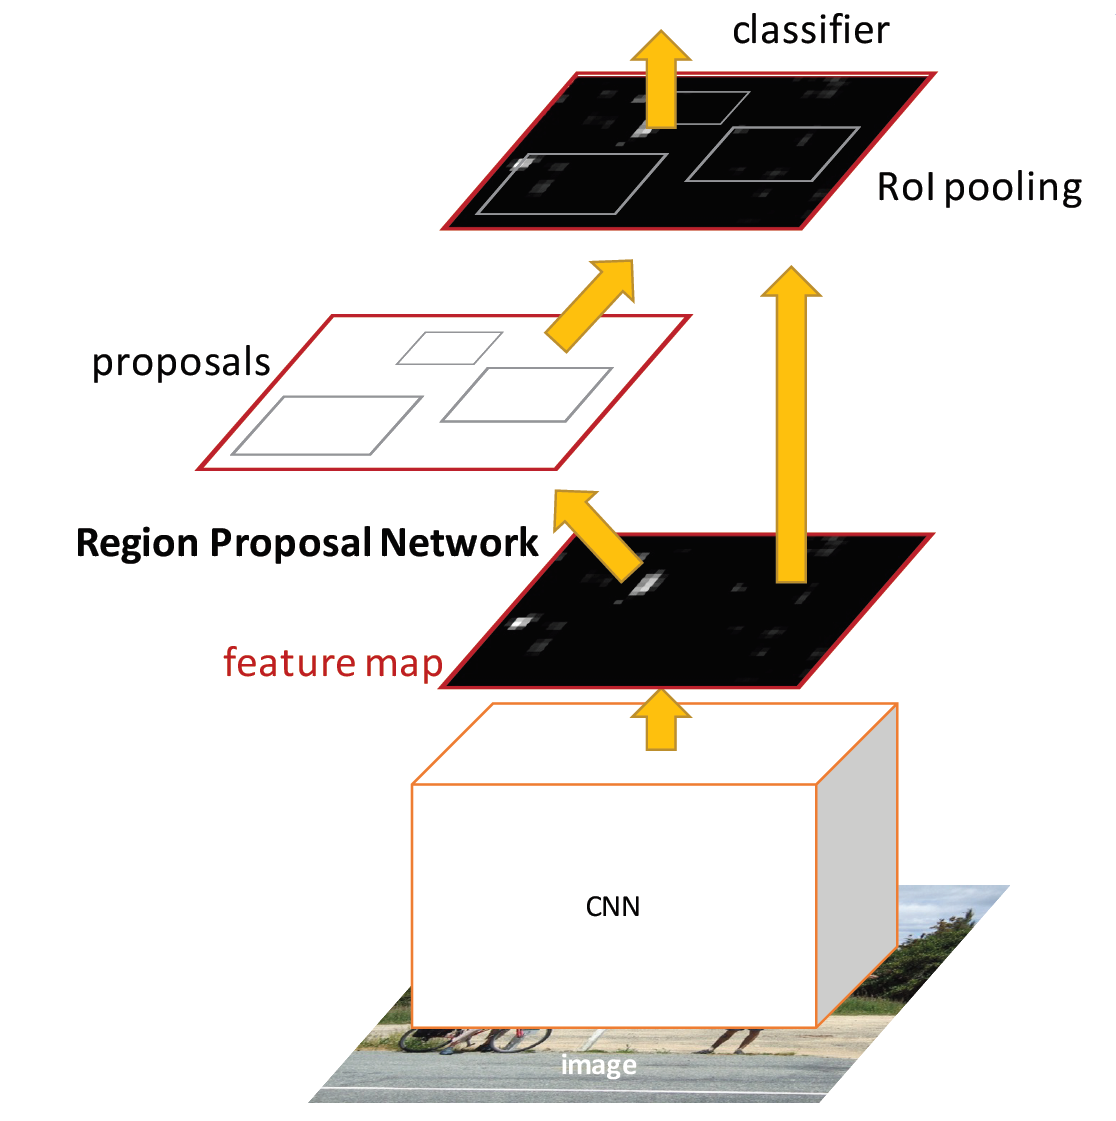
\includegraphics[scale=0.18]{images/FRCN_architecture}
\caption{The Faster R-CNN architecture. Note the weight sharing between RPN Network and the classifier.}
\label{fig:rcnn-architectures}
\end{wrapfigure} we will present the most important ones in the following.\\ In 2015, \textbf{Faster Region-based Convolutional Networks (Faster R-CNNs}, \cite{DBLP:journals/corr/RenHG015}\textbf{)}  have come up as an enhancement  of the existing R-CNN and Fast R-CNN methods that are both based on distinct region proposal networks to find candidate bounding boxes and detection networks to perform classification. Faster R-CNN extend this by introducing weight sharing of the convolutional features between region proposal network and detection network, facilitating nearly cost-free region proposals (see Figure \ref{fig:rcnn-architectures}). 

These methods, being all based on a two-stage process of having one part of their network dedicated to providing region proposals followed by a classifier to classify these proposals, are  very accurate - however, this comes at the expense of inference speed, making them not fit to be used on embedded devices.\\
\begin{wrapfigure}{h}{0.55\textwidth}

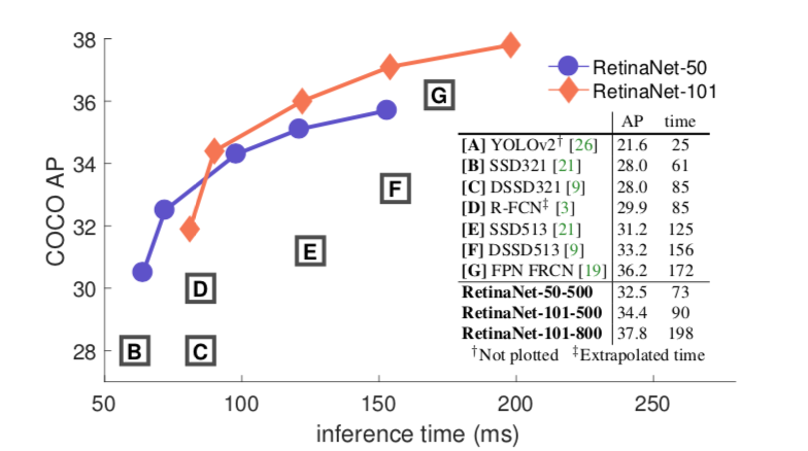
\includegraphics[scale=0.32]{images/retinanet}
\caption{Evaluation of different object detection algorithms on the COCO dataset from the RetinaNet paper. Currently, evaluation performance is dominated by the RetinaNet architecture.}
\end{wrapfigure}
Another way of doing object detection is by combining these two tasks a single unified network, a so-called one-stage detector.



One-stage detectors like \textbf{You Only Look Once (YOLO)} \cite{DBLP:journals/corr/RedmonDGF15}\cite{DBLP:journals/corr/RedmonF16}\cite{DBLP:journals/corr/abs-1804-02767} or \textbf{Single-Shot Detector (SSD)} \cite{DBLP:journals/corr/LiuAESR15} that are applied over a regular, dense sampling of possible object locations have the potential to be faster and simpler, but have trailed the accuracy of two-stage detectors because of extreme class imbalance encountered during training.
In 2016 and 2017, researchers from FacebookAI have developed concepts \cite{DBLP:journals/corr/abs-1708-02002}\cite{DBLP:journals/corr/LinDGHHB16} circumventing this - with the main idea being to reshape cross entropy loss such that it down-weights the loss assigned to well-classified examples. The novel focal loss focuses training on a sparse set of hard examples and prevents the vast number of easy negatives from overwhelming the detector during training. Combining this with the concept of pyramidal networks, in which a top-down architecture with lateral connections is developed for building high-level semantic feature maps at all scales, we get the \textbf{Focal Loss for Dense Object Detection (RetinaNet)} which currently outperformes all other object detection algorithms in terms of performance with state-of-the-art inference times (see Figure 7).

\section{Methods [Frank]}
As we motivated our project with the implementation of our network in embedded devices such as laptop webcams and smartphone cameras, we decided to use the latest iteration of the YOLO algorithm which has come up in April 2018 and still is the fastest object detection algorithm (despite being outperformed by RetinaNet, SSD and RCNN approaches).
\subsection*{The YOLO approach to object detection}
YOLO's general approach is that object detection is re-framed as a single regression problem, directly
modelling bounding box coordinates and class
probabilities from image pixels. This means that the YOLO model only ”looks
once” at an image for object detection.
It works as follows: 
\begin{itemize}
\item[--] divide an image into an $S\times S$ grid
\item[--] in training, each grid cell is responsible for predicting only the bounding boxes whose center pixel falls within them (see Figure \ref{fig:cell})
\item[--]  predict $B$ bounding boxes and a confidence score for each box representing the probability that an object is contained inside a bounding box (often called \textit{objectness score}) as well as a single $C$-dimensional vector of class probabilities, making the output vector $S \times S \times (B\times 5 +C)$-dimensional

\item[--] predictions are made using a technique called non-maximum suppression in which we remove low probability bounding boxes that are very close to high probability bounding boxes. 
\end{itemize}  At test time the conditional class probabilities and the individual box confidence predictions are multiplied, resulting in a feature map of bounding boxes ``weighted'' by their per-class confidence scores (see figure 8).

\begin{SCfigure}
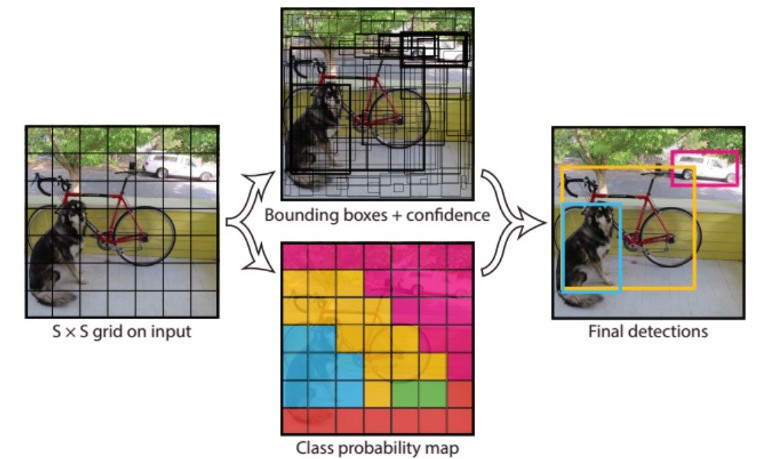
\includegraphics[scale=0.35]{images/yolo_model}\label{fig:yolomodel}
\caption{For each of the $S^2$ grid cells, we make one objectness prediction and four positional predictions for bounding boxes relative to each of the $B$ anchor boxes as well as a global class prediction vector. Combination of these values using NMS grants the final predictions.}
\end{SCfigure}


\subsubsection*{Anchor boxes}
Instead of wildly predicting $B$ bounding boxes per grid cell, the idea of YOLO is to predict offsets to $B$ so-called anchor boxes. Anchor boxes are rectangular boxes that are not learned, but pre-defined before training - the idea being that they should be representative of as many ground-truth bounding boxes as possible. \\
Usually, one sets these boxes beforehand, for example by using the k-means algorithm, grouping together conceivable anchor boxes of objects shapes you tend to get. 
\begin{SCfigure}
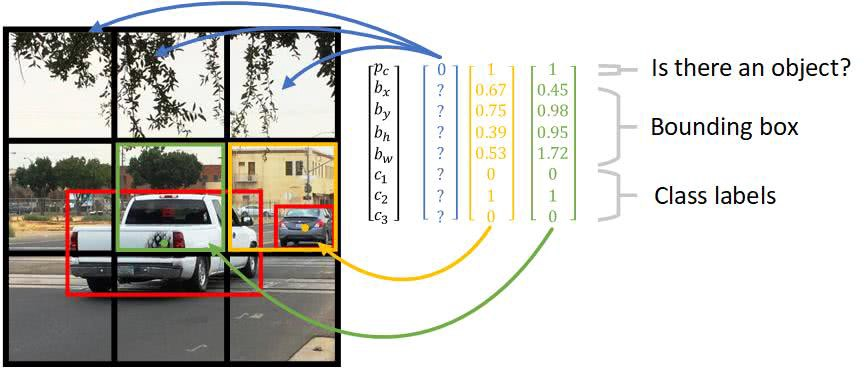
\includegraphics[scale=0.35]{images/yolo_mechanics}
\caption{For each grid cell, we predict vectors of multiple bounding boxes (here, only one bounding box is predicted, $B=1$), but only one class prediction vector of length $C$ (here, $C$=3).}
\label{fig:cell}
\end{SCfigure}



\subsubsection*{Architecture and training hyperparameters}
YOLO is implemented as a 32 layer deep convolutional
neural network. The open source implementation released
along with the paper is built upon a custom DNN
framework written by YOLO’s authors, called darknet, implemented in C.
Several variants of YOLO have been released in the last couple of years. For our purposes, we
chose the variant ``tiny YOLOv3'' which is a simplified version of YOLOv3 for restricted environments such as ours.\footnote{https://github.com/pjreddie/darknet/blob/master/cfg/yolov3-tiny.cfg} (see figure 10). 
\subsubsection*{Loss function}

YOLO’s loss function must optimize the network's parameters as to simultaneously solve the object localization and object classification tasks. This function
simultaneously penalizes incorrect object detections
as well as considers what the best possible classification
would be. The YOLO loss function is designed to simultaneously minimize the sum of squared errors, with scale parameters to control how much we want to increase the loss from bounding box coordinate predictions ($\lambda_\textbf{coord}$) and how much we want to decrease the loss from confidence predictions for boxes that don’t contain objects ($\lambda_\textbf{no\_obj}$) We
implement the following loss function, composed of five
terms:
${\mathbb{1}}_{ij}^{\text{obj}}$ is 1 for the $i$-th grid square and $j$-th bounding box predictor and 0 otherwise ${{\mathbb{1}}}_i^{\text{obj}}$ is 1 if an object appears in the $i$-th cell and 0 otherwise.
$p_i(c)$ and $\hat{p}_i(c)$ represent the actual and predicted conditional probabilities of whether cell i contains an object of class c.
Further, $S$ denotes the number of grid cells, $B$ the number of anchor boxes per grid cell, $w_i$ and $h_i$ width and height and $x_i$ and $y_i$ the mid coordinates of each bounding box.
\begin{align*}
\lambda_\textbf{coord}
\sum_{i = 0}^{S^2}
    \sum_{j = 0}^{B}
     {\mathbb{1}}_{ij}^{\text{obj}}
            \left[
            \left(
                x_i - \hat{x}_i
            \right)^2 +
            \left(
                y_i - \hat{y}_i
            \right)^2
            \right]&\textbf{\ coordinate loss}
\\\\
+ \lambda_\textbf{coord} 
\sum_{i = 0}^{S^2}
    \sum_{j = 0}^{B}
         {\mathbb{1}}_{ij}^{\text{obj}}
         \left[
        \left(
            \sqrt{w_i} - \sqrt{\hat{w}_i}
        \right)^2 +
        \left(
            \sqrt{h_i} - \sqrt{\hat{h}_i}
        \right)^2
        \right]\\
+ \lambda_\textbf{obj}\sum_{i = 0}^{S^2}
    \sum_{j = 0}^{B}
        {\mathbb{1}}_{ij}^{\text{obj}}
        \left(
            C_i - \hat{C}_i
        \right)^2&\textbf{\ objectness loss}
\\
+ \lambda_\textbf{no\_obj}
\sum_{i = 0}^{S^2}
    \sum_{j = 0}^{B}
    {\mathbb{1}}_{ij}^{\text{no\_obj}}
        \left(
            C_i - \hat{C}_i
        \right)^2\\ 
+ \sum_{i = 0}^{S^2}
{{\mathbb{1}}}_i^{\text{obj}}
    \sum_{c \in \textrm{classes}}
        \left(
            p_i(c) - \hat{p}_i(c)
        \right)^2&\textbf{\ classification loss}
\end{align*}



\begin{figure}[h]
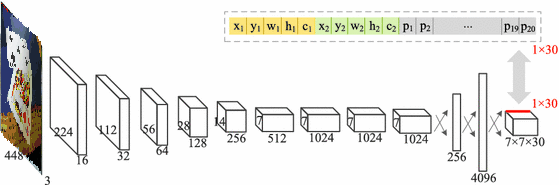
\includegraphics[width=1\linewidth]{images/tinyyolo}
\caption{A simple YOLO-v3 feature extractor with a grid size of $7\times 7$, $B=2$ and 20 classes, making the final prediction vector ($7 \times 7 \times 30$) - dimensional. }
\end{figure}
\newpage


\section{Webcam deployment [Frank \& Daniel]}
To test the performance of our network and getting into real-life applications, we needed a solution running on a computer to deliver the recognition results. We deployed tinyYOLO on a webcam using a (rather slow) GPU (GeForce GTX 960M) getting about 35 FPS depending on brightness levels, which is essentially real-time. To achieve this, we used the capabilities of the Python implementation of \textit{OpenCV}, particularly making use of the \textit{VideoCapture} class.

\section{Evaluation [Frank \& Daniel]}
Each model is judged by its performance on a test set that is never seen by the training algorithm. For each application, it is critical to find a metric that can be used to objectively compare models.
Evaluation in object detection is made more difficult due to localization and classification being distinct tasks needing to be optimized.  
In literature, the most widely used approach for evaluating localization and classification is mean average precision (mAP).  \\
The first main idea for this approach, is to judge how well the detection was performed.  For this, we measure the intersection of the Bounding Box detection with the ground truth, over the the union of both.  This rate (so called IoU), let us designate our detection as True Positive, if the IoU is greater than a fix threshold value, or False Positive otherwise.
Having calculated this for each image on the validation set, we can talk about how well the detection was.  A quantity for this is given by the so called Precision, which is given by:
\[\text{Precision} = \frac{\text{True Positives}}{\text{True Positives}+\text{False Positives}}, \]
where Precision $\in [0,1]$ has a higher value when the detection was well performed and a low value otherwise.
We can compute the Precision for each class and then take the average of this.  This bring us to the Average Precision. \\
Notice that for this computations, we fixed a threshold value for the IoU.   In order to get the mAP, we compute the Precision of each class varying at a set of eleven equally spaced levels 
$[0, 0.1, 0.2, ... , 1]$, and after this computing the mean of them. 
An equivalent way of 

\section{Results [Frank \& Daniel]}
Our object detection endeavours using a tiny YOLOv3 detector resulted in diverse results depending on the complexity and pecularities of the synthesized dataset in use - the main results are summarize in table \ref{tab:res}. In termns of mAP, we generally achieved the best results for the datasets without using background textures and only simple transformations (\textbf{mAP $=99.1 \%$}). However, comparing mAPs across different datasets is not very sensible - our test sets were composed of 5 \% random samples from the particular dataset that we had trained on which made it a lot easier for the ``earlier'' datasets as their test set was comparably easy.

In total, training always converged rather quickly (see Figure 11).\\
\begin{SCfigure}

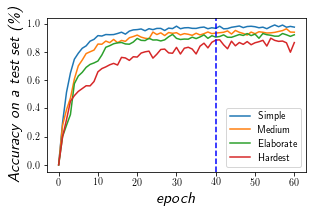
\includegraphics[scale=1]{images/loss}
\label{fig:curve}
\caption{Precision values (for a IOU threshold of 0.5) after each training epoch evaluated on the test set pertaining to the dataset being trained on. As you would expect, the easier the dataset, the faster the training and the better the results. }


\end{SCfigure}
\begin{table}[h]


\begin{tabular}{lllllr}
\hline
\multicolumn{5}{c}{Dataset situation} \\
\cline{1-2}
name    & description  & precision & recall & mAP \\
\hline
\textbf{1 - Simple}      & Paste cards on simple canvases    &  0.974  & 0.996 & \textbf{0.991} \\
          & \textit{random rotations, brightness, blurring}     & & & \\
\textbf{2 - Medium}      & Paste randomly scaled cards on simple canvases & 0.946 & 0.988 & \textbf{0.989} \\
          & \textit{random rotations, brightness, blurring}     & & & \\
\textbf{3 - Elaborate}       & Paste randomly scaled cards on textures & 0.937 & 0.978 & \textbf{0.971} \\
          & \textit{random rotations, brightness, blurring}     & & & \\
\textbf{4 - Hardest} & Paste randomly scaled cards on textures & 0.940 & 0.983 & \textbf{0.973} \\
          & \textit{random rotations, brightness, blurring, less zoom}     & & & \\
\hline


\end{tabular}
\caption{Precision and recall values have been calculated using a IOU threshold of 0.5. mAP values are based on averaged precision values over IOU thresholds of $[0.1, 0.2, \dots 0.8, 0.9] $  }
\label{tab:res}
\end{table}
\subsection*{Exemplary test results and failure cases}

\begin{figure}[h]

\begin{tabular}{ccc}

 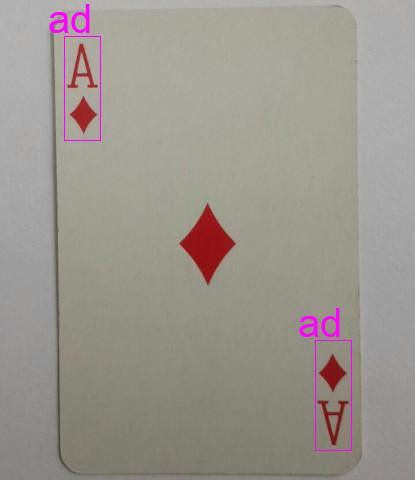
\includegraphics[height=44mm]{images/ad} &   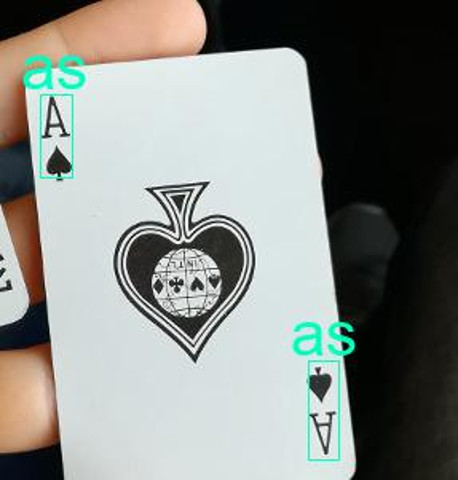
\includegraphics[height=44mm]{images/as} &   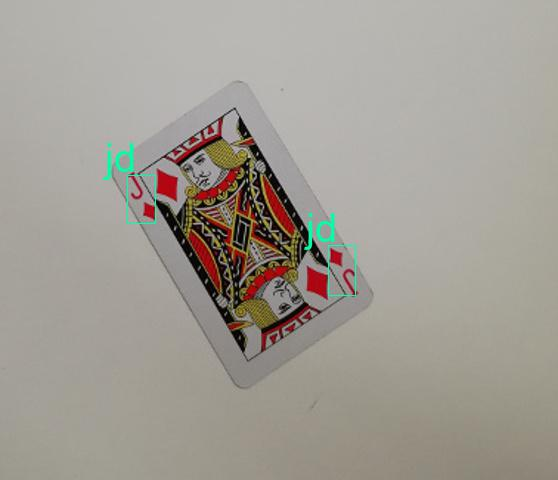
\includegraphics[height=44mm]{images/jd}\\
\makecell{\textbf{success:} classification: \\ \textbf{Ad:} 0.99995, \textbf{Ad:} 0.99997}  & \makecell{\textbf{success:}  classification \\ \textbf{As:} 0.99757, \textbf{As:} 0.99931} & \makecell{\textbf{success:}  classification \\ \textbf{Jd:} 0.99967, \textbf{Jd:} 0.99992}\\[6pt]




\end{tabular}
\caption{Successful cases of detection of images that are pretty representative of the training distribution}
\label{fig:testcases}
\end{figure}

Metrics are most helpful in measuring the effectiveness of algorithms, but more often than not, computer vision tasks allow for an additional visual inspection of results. \\Hence, we compiled a couple of results on unseen test images (see figure \ref{fig:testcases}).
\begin{figure}[h]

\begin{tabular}{ccc}

 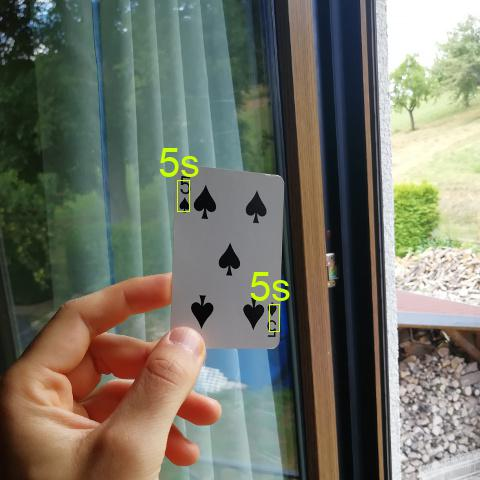
\includegraphics[width=44mm]{images/success3} &   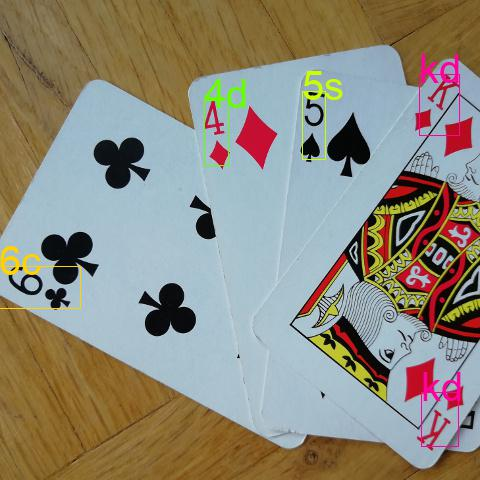
\includegraphics[width=44mm]{images/success2} &   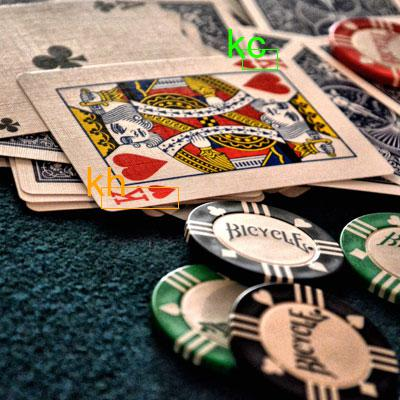
\includegraphics[width=44mm]{images/success1}\\
\makecell{\textbf{success:} scenario with a \\ highly diverse background \\ \textbf{5s:} 0.99932 \textbf{5s:} 0.95450
}  & \makecell{\textbf{success:}  multiple cards \\ with trivial background \\ \textbf{Kd}: 0.99999 \textbf{Kd}: 0.99994\\
\textbf{4d}: 0.98266
\textbf{5s}: 0.90017\\
\textbf{6c}: 0.99985
} & \makecell{\textbf{success:}  angled shot of sheared card \\ in front of highly diverse background \\\textbf{Kh:} 0.978553
\textbf{Kc:} 0.448083
}\\[6pt]
  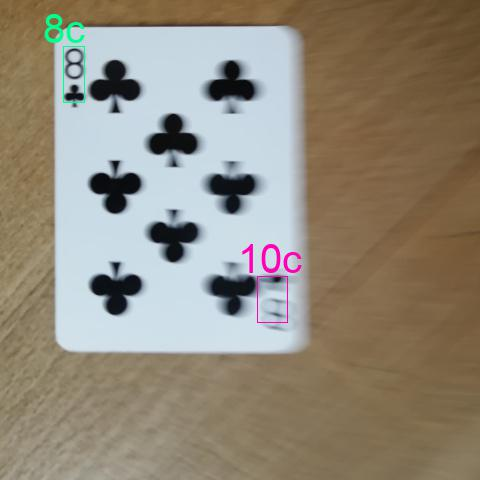
\includegraphics[width=44mm]{images/fail1} &   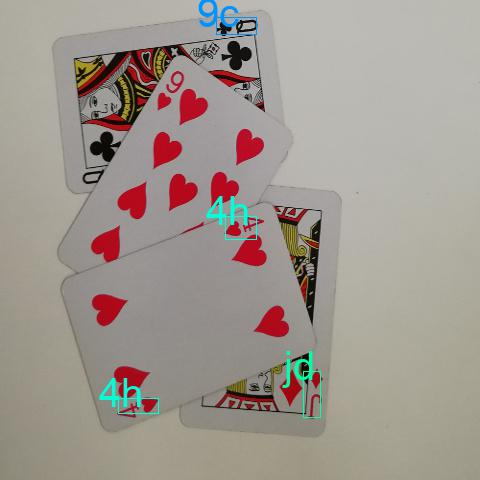
\includegraphics[width=44mm]{images/fail2} &   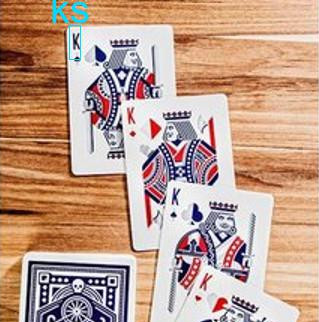
\includegraphics[width=44mm]{images/fail3}\\
\makecell{\textbf{fail:}  misdetection of 8c \\ due to motion blur \\\textbf{8c:} 0.998637
\textbf{10c:} 0.343506
} & \makecell{\textbf{fail:} misdetection of Qc and non- \\detection of 9h for unknown reason \\
\textbf{4h:} 0.972108
\textbf{4h:} 0.830992\\
\textbf{9c:} 0.652040
\textbf{Jd:} 0.241018} & \makecell{\textbf{fail:} very confused model \\ due to wildly different distribution \\ \textbf{Ks:} 0.901385
\textbf{Ks:} 0.612234\\
\textbf{Kc:} 0.640308
\textbf{Kh:} 0.452825
} \\[6pt]



\end{tabular}
\caption{Successful cases of detection (top row) and typical fail cases (bottom row) along with corresponding classification scores.}
\label{fig:testcases}
\end{figure}
Generally, as was to be expected, the predictions were pretty good when the test images were \textit{somewhat} representative of the training data. This is not of particular interst
When multiple cards were present in an image, it was a tough task to find a completely correctly classified image than to find one that our model did some mistakes on (middle column) as we trained on images with single cards only. Yet, in images with only one card, our model seems quite robust, at least if there is not too much blurring or other types of cluttering going on. Also, as we trained on a single deck of cards, it seems natural that the model has problems with predicting cards coming from completely different decks.
\subsection*{Results of further work}
\subsubsection*{Transfer learning}
For all of the experiments above, we started training using a network pre-trained on the VOC dataset \cite{Everingham15}\footnote{PyTorch weights are available at \url{https://pjreddie.com/media/files/yolov3-tiny.weights}.}. After having trained our network on our own dataset, we also experimented with using our own fine-tuned weights from previous datasets for training subsequent models. This generally led to distinctly faster convergence which makes sense as the distribution of weights for similar datasets will obviously be similar. However, this was not much of a concern as the training procedure was fast and large speed-ups were not needed.
\subsubsection*{Webcam deployment}
Depending on the scenery, our model running on a laptop webcam resulted in satisfactory to good results.
\section{Discussion and Future Work [Frank \& Daniel]}
\subsection*{Overview}
Using an artificially created annotated dataset of playing cards in situations reflecting realistic scenarios as good as possible, we perform object detection using the YOLOv3 object detection algorithm, achieving a mAP score of 97.30\% on a holdout dataset. \\ 
Two things are worth noticing in particular: 
 First, datasets without complex textures ("Simple", "Medium") led to better (i.e. faster) convergence (see Figure 11). This intuitively makes sense as the algorithm does not need to spend time ruling out complex dependencies that might be learned from unimportant pixels or regions outside the card. Second, the training procedure experienced much more variance as complexities of the datasets increased, which can be explained by the training algorithm having to deal with much more complex data manifolds and it being possibly hung up in local minima much more which it has to navigate out of. \\
 Testing our model using self-taken photographs of playing cards worked really well for the general dataset (see Figure 12). Obviously, due to not having trained on images with multiple cards and a variation of different decks of cards, these scenarios exacerbate the task greatly (see Figure 13).
\subsubsection*{Training process}
The training procedure went rather swiftly. Apparently,  the particular task of detecting ranks/suits of playing cards is easy for our model - it can be thought of as 2D rather than 3D - in the end, playing cards are flat pieces of paper that do not show much variation in a 3D-world unlike other natural objects where algorithms have to learn representations of varying angle and shadow conditions or situations involving occlusion and the likes. \\
\subsubsection*{Deployment on a webcam}
Testing our model on a webcam resulted in satisfactory,  results. In many scenarios, especially with very bright backgrounds, the ``black'' suits \textit{clubs} and \textit{spades} dominated the scenery and were generally easier to be detected. Apparently, our dataset and corresonding transformations are not be general enough to cover the kinds of images captured by a stock laptop webcam. Light backgrounds cause the color channels of RGB images to be weakened. If a model relies on color information too much, it will subsequently confuse, for example, hearts with spades, due to them having very similar shapes.

\subsection*{Future Work [Frank]}
Our model works very well in the limited domain described above. However, if we were to develop a more reliable system, there are several extensions to be made.
\begin{description}
\item[more general dataset] The probably largest room for improval lies in the generation of a more general dataset - we trained on a single deck of cards, using one set of photographs. A more reliable approach would be to train on several decks of cards, include more than one card per image, use more actual photos of more realistic lighting situations, use realistic images as backgrounds instead of textures etc.
Also, we did not include the realistic scenario of shadows in the dataset at all, which also compromises generalisability.
\item[more thorough hyperparameter search] There are several hyperparameters of YOLO. We unsystematically experimented with changing the anchor box sizes, learning rate and grid size without experiencing greatly improved results. A more thorough hyperparameter (grid) search might warrant better results.

\item[explore other architectures] Quite possibly, the inclusion of a more general dataset would cause tiny YOLOv3 to be overwhelmed. While small architectures are beneficial to training and inference times as well as decreasing the risk of overfitting, they also encounter difficulties when relationships to be learned become overly complex. Especially including images with a very large range of scaling/zoom introduces a large number of more subtelities to be learned.
\item[cross-validation] We tested our model on a fixed set of test images. While there is nothing wrong with this approach, we might want to get estimates of test performance encompassing less variance. Performing, say, 10-fold cross-validation would warrant that. However, due to our capability to generate test data essentially for free, cross-validation is not the only tool to decrease test variance.
\item[error analysis] In order to improve an object detection model, a single scalar such as mAP does not quite suffice - to do this properly, we would have to compare precision and recall values for each class separately and optimize thresholding values. As our work is merely a proof-on-concept with very constrained time limit, we desisted from work towards that for now.
\item[extending the cheating pipeline] A system to recognize playing cards is only one part of the big task of effective cheating. The ways in which a system like ours may be used are manifold: for one, one might deploy it into a smart contact lense or smart glasses in order to augment a user's reality with information based on what cards have been seen or, much more evil, might use fixed surveillance cameras in the room to detect cards of opponents and feed this information back to the cheating player.
\end{description}

\section{Conclusion  [Frank \& Daniel]}
Using the YOLOv3 object detection algorithm, we managed to detect the suits and ranks of playing cards in a general setting. As our project was conceived to be a proof-of-concept - in order to build a model that is actually able to help people cheat effectively, several extensions would need to be made to our approach, which are mainly comprised of coming up with a more general dataset. \\ Also, the lack of commodity contact lenses equipped with video cameras and GPUs in close proximity would currently aggravate deployment - until then, card game players are protected from this kind of fraud.
\\The project files, mock datasets and, prospectively, further development are available at\\ \url{https://github.com/DanielGonzalezAlv/PlaycDC.git}.

\newpage
 \bibliographystyle{acm}

\bibliography{cite}
\end{document}
